% Laporan IF4031 Milestone 1 -- ARGUS: Aggregated Real-time Geohazard Unified System
% Kompilasi: tectonic -X compile main.tex   (atau xelatex main.tex dua kali)
% Berkas keluaran diganti nama menjadi IF4031_M1_<NamaKelompok>.pdf saat dikumpulkan.
\documentclass[11pt,a4paper,oneside]{report}
\usepackage{fontspec}
\setmainfont{texgyrepagella}[Extension=.otf,UprightFont=*-regular,BoldFont=*-bold,ItalicFont=*-italic,BoldItalicFont=*-bolditalic]
\setsansfont{texgyreheros}[Extension=.otf,UprightFont=*-regular,BoldFont=*-bold,ItalicFont=*-italic,BoldItalicFont=*-bolditalic,Scale=MatchLowercase]
\setmonofont{lmmono10-regular}[Extension=.otf,BoldFont=lmmonolt10-bold,ItalicFont=lmmono10-italic,BoldItalicFont=lmmonolt10-boldoblique,Scale=MatchLowercase]
\usepackage[indonesian]{babel}
\usepackage[a4paper,margin=2.4cm,headheight=14pt]{geometry}
\usepackage{microtype}
\usepackage{setspace}
\setstretch{1.12}
\usepackage{parskip}
\setlength{\parskip}{0.55em}
\usepackage{xcolor}
\usepackage{booktabs,tabularx,array,longtable,multirow}
\usepackage{enumitem}
\setlist{nosep,leftmargin=1.4em,itemsep=0.2em}
\usepackage{url}
\urlstyle{tt}
\makeatletter
\g@addto@macro\UrlBreaks{\do\_\do\=\do\:\do\,}
\g@addto@macro\UrlBigBreaks{\do\_\do\[\do\]\do\(\do\)}
\makeatother
\Urlmuskip=0mu plus 0.5mu
\emergencystretch=2.5em
\usepackage{listings}
\usepackage{tikz}
\usetikzlibrary{positioning,fit,backgrounds,arrows.meta,shapes.geometric,calc}
\usepackage[most]{tcolorbox}
\usepackage{fancyhdr}
\usepackage{titlesec}
\usepackage{caption}
\usepackage[hidelinks]{hyperref}

% ---- warna
\definecolor{ink}{HTML}{1F2933}
\definecolor{accent}{HTML}{1F4E79}
\definecolor{accentlight}{HTML}{E8F0F8}
\definecolor{okgreen}{HTML}{1E7B4F}
\definecolor{okbg}{HTML}{E7F5EE}
\definecolor{warnorange}{HTML}{B35C00}
\definecolor{warnbg}{HTML}{FFF3E0}
\definecolor{todored}{HTML}{B00020}
\definecolor{gridgray}{HTML}{8A97A3}
\definecolor{codebg}{HTML}{F4F6F8}
\color{ink}

% ---- judul bagian
\titleformat{\chapter}[hang]{\sffamily\bfseries\huge\color{accent}}{\thechapter}{0.6em}{}
\titlespacing*{\chapter}{0pt}{-10pt}{22pt}
\titleformat{\section}{\sffamily\bfseries\Large\color{accent}}{\thesection}{0.6em}{}
\titleformat{\subsection}{\sffamily\bfseries\large\color{ink}}{\thesubsection}{0.6em}{}
\titleformat{\subsubsection}{\sffamily\bfseries\normalsize\color{ink}}{}{0em}{}
\titlespacing*{\section}{0pt}{1.6em}{0.5em}
\titlespacing*{\subsection}{0pt}{1.2em}{0.4em}

% ---- header/footer
\pagestyle{fancy}
\fancyhf{}
\renewcommand{\headrulewidth}{0.3pt}
\fancyhead[L]{\sffamily\footnotesize IF4031 -- Laporan Milestone 1}
\fancyhead[R]{\sffamily\footnotesize BNPB Disaster Coordination Gateway}
\fancyfoot[C]{\sffamily\footnotesize\thepage}

% ---- tampilan kode / log
\lstset{
  basicstyle=\ttfamily\scriptsize,
  backgroundcolor=\color{codebg},
  frame=single, rulecolor=\color{gridgray!50},
  breaklines=true, breakatwhitespace=false,
  columns=fullflexible, keepspaces=true,
  xleftmargin=2pt, xrightmargin=2pt,
  aboveskip=0.6em, belowskip=0.4em,
  upquote=true
}
% \code: tanpa spasi, boleh putus baris di / _ - . ; \cmd: mempertahankan spasi (perintah terminal).
\newcommand{\code}[1]{\path{#1}}
\newcommand{\cmd}[1]{\texttt{\detokenize{#1}}}
\newcommand{\todo}[1]{\textcolor{todored}{\textbf{[#1]}}}

% ---- kotak
\newtcolorbox{ringkas}[1][Singkatnya]{
  enhanced, breakable, colback=accentlight, colframe=accent, boxrule=0.5pt,
  left=6pt,right=6pt,top=4pt,bottom=4pt, fonttitle=\sffamily\bfseries\small, title={#1}}
\newtcolorbox{jawaban}[1][Jawaban butir ``Di laporan'']{
  enhanced, breakable, colback=okbg, colframe=okgreen, boxrule=0.5pt,
  left=6pt,right=6pt,top=4pt,bottom=4pt, fonttitle=\sffamily\bfseries\small, title={#1}}
\newtcolorbox{catatan}[1][Catatan jujur]{
  enhanced, breakable, colback=warnbg, colframe=warnorange, boxrule=0.5pt,
  left=6pt,right=6pt,top=4pt,bottom=4pt, fonttitle=\sffamily\bfseries\small, title={#1}}

% ---- tabel
\renewcommand{\arraystretch}{1.18}
\newcolumntype{L}[1]{>{\raggedright\arraybackslash}p{#1}}
\newcolumntype{Y}{>{\raggedright\arraybackslash}X}
\captionsetup{font={small,sf},labelfont=bf,skip=4pt}
\newcommand{\lulus}{\textcolor{okgreen}{\textbf{Lulus}}}
\newcommand{\sebagian}{\textcolor{warnorange}{\textbf{Sebagian}}}
\newcommand{\belum}{\textcolor{todored}{\textbf{Belum}}}

\usepackage{graphicx}
\usepackage{float}
\usepackage{pdfpages}

\begin{document}

% =============================================================== sampul
\begin{titlepage}
\thispagestyle{empty}
\sffamily
\vspace*{1.2cm}
{\color{accent}\rule{\textwidth}{1.6pt}}\\[1.2em]
{\Large IF4031 Arsitektur Aplikasi Terdistribusi}\\[0.4em]
{\large Tugas Besar -- Milestone 1: Sistem Terdistribusi Dasar}\\[2.2em]
{\fontsize{40}{44}\selectfont\bfseries\color{accent} ARGUS}\\[0.5em]
{\Large\bfseries Aggregated Real-time Geohazard Unified System}\\[0.8em]
{\large Gateway koordinasi kebencanaan BNPB yang menyatukan data BMKG dan PVMBG}\\[1.2em]
{\color{accent}\rule{\textwidth}{0.6pt}}

\vspace{2.2cm}
\begin{tabular}{@{}L{3.6cm}L{10cm}@{}}
\textbf{Nama kelompok} & OrangSuksesAamiin\\[0.8em]
\textbf{Anggota} & 13523128 - Andi Farhan Hidayat\\
 & 13523164 - Muhammad Rizain Firdaus\\
 & 13523152 - Muhammad Kinan Arkansyaddad\\[0.8em]
\textbf{Mata kuliah} & IF4031 Arsitektur Aplikasi Terdistribusi\\
\textbf{Institusi} & Institut Teknologi Bandung\\
\textbf{Semester} & 7, 2026/2027
\end{tabular}

\vfill
{\small\color{gridgray}Berkas ini dikumpulkan sebagai \texttt{IF4031\_M1\_OrangSuksesAamiin.pdf}.}
\end{titlepage}

% =============================================================== isi
\pagenumbering{roman}
\tableofcontents
\clearpage
\pagenumbering{arabic}

\chapter{Bagian Umum}

\section{Tabel kontribusi}

Tabel ini menunjukkan siapa mengerjakan apa. Pembagian kerja mengikuti tiga tahap: fondasi dan Problem~1, lalu
Problem~2 dan~3, lalu Problem~4 dan~5 beserta integrasi.

\begin{table}[!htbp]
\centering
\small
\begin{tabularx}{\textwidth}{@{}L{2.9cm}YYY@{}}
\toprule
\textbf{Anggota} & \textbf{Perancangan} & \textbf{Implementasi} & \textbf{Penulisan laporan}\\
\midrule
Orang~1 \newline Andi Farhan Hidayat &
 Kontrak antar-komponen, arsitektur Aggregator, kebijakan skema &
 Fondasi (\code{pkg/obs}, Compose, Makefile, CI), mock BMKG dan PVMBG, Aggregator, Problem~1, ketahanan ingest, adapter PostgreSQL dan Kafka, outbox dan relay, consumer &
 Bagian umum, Problem~1, deskripsi mock\\
Orang~2 \newline Muhammad Rizain Firdaus &
 Autentikasi JWT tiga peran, kebijakan field Ringkasan/Mentah, pembatas laju, penanda \code{stale} &
 \code{auth-service}, \code{client-api}, skrip demo dan load test Problem~2 dan~3 &
 Problem~2, Problem~3\\
Orang~3 \newline Muhammad Kinan Arkansyaddad &
 Perbandingan pilihan penyimpanan (PostgreSQL dengan JSONB) dan pilihan penyebaran event (Kafka dengan outbox), semantik pengiriman, dan batasan yang disadari &
 Skrip demo Problem~4 dan~5 (membangun ulang satu service, field baru tanpa migrasi, consumer baru) dan pengujian pemulihan consumer &
 Problem~4, Problem~5\\
\bottomrule
\end{tabularx}
\caption{Kontribusi anggota.}
\end{table}

\section{Deskripsi umum sistem}

Di cerita soal, Astolfo menerima sinyal bencana dari banyak lembaga yang tidak saling bicara. Sistem ini, ARGUS
(\emph{Aggregated Real-time Geohazard Unified System}), adalah \emph{gateway} milik BNPB yang menyambungkannya. Ia melakukan lima hal:

\begin{enumerate}
 \item \textbf{Mengambil} data dari dua lembaga secara berkala (\emph{polling}): BMKG untuk gempa dan tsunami, PVMBG untuk gunung api.
 \item \textbf{Menyeragamkan} dua format yang berbeda menjadi satu format milik BNPB, yaitu \emph{HazardEvent}.
 \item \textbf{Menyimpan} hasilnya di satu penyimpanan, \emph{Canonical Store}, yang hanya dikelola oleh satu service.
 \item \textbf{Menyebarkan} setiap data baru ke pihak yang berlangganan lewat \emph{message broker}.
 \item \textbf{Menyajikan} data ke tiga jenis klien (Media, Tim Lapangan, BNPB Pusat) dengan hak akses yang berbeda.
\end{enumerate}

\textbf{Lingkup Milestone 1} dibatasi oleh soal: dua lembaga sumber (BMKG dan PVMBG), dua jenis bencana (seismik dan
vulkanik), BNPB sebagai simpul koordinasi, dan semua klien hanya membaca (\emph{read-only}). BMKG dan PVMBG adalah
\emph{mock} buatan kelompok yang mengikuti kontrak di soal tanpa mengubahnya.

\subsection*{Status penyelesaian}

Tabel berikut merangkum apa yang sudah terbukti lewat demo. Bukti P1 dan sisi ingest P2 dibuat pada 7~Oktober~2026;
bukti sisi layanan P2, P3, P4, dan P5 pada 8~Oktober~2026. Demo P2 dan P3 dijalankan sekali setelah \cmd{make reset}.
Demo P4 dan P5 dijalankan setelah reset dan diulang sekali tanpa reset; keduanya lulus kedua kali.

\begin{table}[!htbp]
\centering
\small
\begin{tabularx}{\textwidth}{@{}L{3.0cm}Y L{2.0cm}@{}}
\toprule
\textbf{Problem} & \textbf{Yang sudah terbukti $\;/\;$ yang masih kurang} & \textbf{Status}\\
\midrule
P1 Interoperabilitas data & Pemetaan benar, skema PVMBG berubah saat berjalan tanpa restart, field baru masuk \code{attributes}, perubahan yang tidak didukung dikarantina. & \lulus\\
P2 Konkurensi dan ketersediaan & p95 BMKG-only di bawah 300~ms saat PVMBG 3~detik, load test 50~koneksi selama 60~detik, outage PVMBG ditangani, pulih tanpa restart. & \lulus\\
P3 Autentikasi dan kepercayaan & Kredensial antar-lembaga saling menolak, Media hanya Ringkasan, token Lapangan kedaluwarsa lalu di-\emph{refresh}, tidak ada kredensial ter-commit. & \lulus\\
P4 Microservice dan storage & Satu container (\code{pvmbg-mock}) dihentikan, dibangun ulang, dan dijalankan lagi tanpa menyentuh yang lain; field baru masuk JSONB tanpa migrasi dan record lama tetap terbaca; Canonical Store hanya terjangkau oleh Aggregator. & \lulus\\
P5 Pub/sub & Event lewat Kafka, dua consumer independen, satu consumer dimatikan lalu menyusul event yang tepat, dan consumer ketiga ditambahkan saat sistem berjalan tanpa mengubah producer. & \lulus\\
\bottomrule
\end{tabularx}
\caption{Status per problem pada saat laporan ini ditulis.}
\end{table}

\section{Diagram arsitektur}

Gambar~\ref{fig:arsitektur} memperlihatkan seluruh service, protokol, kepemilikan penyimpanan, dan batas jaringan.

% Gambar 1.1 -- arsitektur sistem. Dipanggil dari umum.tex.
\begin{figure}[!htbp]
\centering
\resizebox{\textwidth}{!}{%
\begin{tikzpicture}[
  font=\sffamily\footnotesize,
  svc/.style={draw=accent, fill=white, rounded corners=3pt, thick, align=center, minimum height=1.05cm, inner sep=4pt},
  mock/.style={svc, draw=gridgray, fill=gray!8},
  store/.style={draw=okgreen, fill=okbg, thick, cylinder, shape border rotate=90, aspect=0.25, align=center, minimum height=1.4cm, minimum width=2.6cm},
  zone/.style={draw=gridgray, dashed, rounded corners=6pt, inner sep=8pt},
  flow/.style={-{Stealth[length=2.2mm]}, thick, color=ink},
  dotflow/.style={-{Stealth[length=2.2mm]}, thick, dotted, color=ink},
  lab/.style={font=\sffamily\scriptsize, color=ink, fill=white, inner sep=1.5pt, align=center}
]
% ---- instansi sumber
\node[mock] (bmkg) at (0,6.4) {\textbf{bmkg-mock}\\:8081 \;\texttt{X-BMKG-Key}};
\node[mock] (pvmbg) at (0,3.6) {\textbf{pvmbg-mock}\\:8082 \;\texttt{Bearer pvmbg.v1...}};
% ---- aggregator
\node[svc, fill=accentlight, minimum width=3.9cm, minimum height=3.1cm] (agg) at (6.4,5.0)
  {\textbf{aggregator}\\[2pt]polling per sumber\\pemetaan ke HazardEvent\\outbox + relay\\API internal :8083};
% ---- sisi klien
\node[svc] (client) at (13.4,8.6) {\textbf{Klien}\\Media $\cdot$ Lapangan $\cdot$ Pusat};
\node[svc] (auth) at (9.2,8.6) {\textbf{auth-service}\\:8084};
\node[svc] (capi) at (13.4,5.6) {\textbf{client-api}\\:8080};
% ---- penyimpanan dan broker
\node[store] (pg) at (6.4,0.4) {\textbf{PostgreSQL}\\Canonical Store};
\node[svc] (kafka) at (10.6,1.7) {\textbf{Kafka}\\topic \texttt{hazard.events}};
\node[svc] (c1) at (14.0,2.9) {\textbf{consumer-dashboard}\\:8091};
\node[svc] (c2) at (14.0,0.5) {\textbf{consumer-notifier}\\:8092};
% ---- zona jaringan
\begin{scope}[on background layer]
 \node[zone, fit=(pg), label={[font=\sffamily\scriptsize,color=gridgray]below:canonical-net (internal)}] {};
 \node[zone, fit=(kafka)(c1)(c2), label={[font=\sffamily\scriptsize,color=gridgray]below:broker-net (internal)}] {};
\end{scope}
% ---- panah
\draw[flow] (agg.west |- bmkg.east) -- (bmkg.east) node[lab, pos=0.45] {poll HTTP};
\draw[flow] (agg.west |- pvmbg.east) -- (pvmbg.east) node[lab, pos=0.45] {poll HTTP};
\draw[flow] (agg.south) -- (pg.north) node[lab, pos=0.5] {baca / tulis};
\draw[flow] (agg.south east) -- (kafka.west) node[lab, pos=0.45] {outbox $\rightarrow$ publish};
\draw[flow] (kafka.east) -- (c2.west);
\draw[flow] (kafka.east) -- (c1.west);
\draw[flow] (client) -- (capi) node[lab, pos=0.5] {Bearer JWT};
\draw[flow] (client) -- (auth) node[lab, pos=0.5] {token / refresh};
\draw[dotflow] (auth.south east) -- (capi.north west) node[lab, pos=0.5] {kunci JWT\\sama};
\draw[flow] (capi.west) -- (capi.west -| agg.east) node[lab, pos=0.5] {\texttt{X-Service-Key}};
\end{tikzpicture}}
\caption{Arsitektur sistem. Garis tegas: panggilan jaringan; garis titik: rahasia penandatangan token yang dipakai bersama. Kotak putus-putus: jaringan Docker yang tidak bisa dijangkau dari luar (\texttt{internal}).}
\label{fig:arsitektur}
\end{figure}


\subsection*{Penjelasan}

\textbf{Alur masuk.} \code{aggregator} memanggil \code{bmkg-mock} dan \code{pvmbg-mock} lewat HTTP. Kedua mock pasif: mereka
hanya menjawab, tidak mengirim data sendiri. Setiap sumber punya putaran polling sendiri, sehingga PVMBG yang lambat
tidak menahan BMKG (Problem~2). Hasil polling dipetakan ke \emph{HazardEvent} dan disimpan.

\textbf{Penyimpanan.} Canonical Store adalah PostgreSQL yang hanya berada di jaringan \code{canonical-net}. Jaringan itu
hanya berisi \code{aggregator} dan database-nya, jadi service lain secara fisik tidak bisa menyambung ke database
(Problem~4). Service lain memperoleh data lewat API internal Aggregator.

\textbf{Alur keluar ke klien.} Klien meminta token ke \code{auth-service}, lalu memanggil \code{client-api} dengan token
itu. \code{client-api} memeriksa token, menentukan field apa yang boleh dilihat peran tersebut, dan meneruskan
permintaan ke API internal Aggregator memakai \code{X-Service-Key}. \code{client-api} tidak pernah memanggil BMKG
atau PVMBG (Problem~2 dan~3).

\textbf{Alur event.} Saat Aggregator menyimpan perubahan, ia menulis juga satu baris \emph{outbox} dalam transaksi
database yang sama. Proses \emph{relay} lalu mengirim baris itu ke topic Kafka \code{hazard.events}. Consumer
berlangganan ke topic tersebut tanpa diketahui Aggregator (Problem~5). Setiap alur membawa \emph{correlation ID} yang
sama dari siklus polling sampai ke consumer.

\subsection*{Daftar container}

Sistem terdiri dari sepuluh container, satu di antaranya hanya tugas sekali jalan. Tabel berikut merangkum port, jaringan, dan penyimpanan masing-masing.

\begin{table}[!htbp]
\centering
\small
\begin{tabularx}{\textwidth}{@{}L{3.7cm}L{2.5cm}L{2.5cm}Y@{}}
\toprule
\textbf{Container} & \textbf{Port host} & \textbf{Jaringan} & \textbf{Penyimpanan yang dimiliki}\\
\midrule
\code{bmkg-mock} & 8081 & app-net & tidak ada (data simulasi di memori)\\
\code{pvmbg-mock} & 8082 & app-net & tidak ada (data simulasi di memori)\\
\code{aggregator} & 127.0.0.1:8083 & app, canonical, broker & Canonical Store (tabel \code{hazards}, \code{outbox}, \code{poll_cursor})\\
\code{postgres-canonical} & tidak dibuka & canonical-net & volume \code{canonical-pgdata}\\
\code{kafka} & tidak dibuka & broker-net & volume \code{kafka-data}\\
\code{kafka-init} & -- & broker-net & tugas sekali jalan: membuat topic\\
\code{auth-service} & 8084 & app-net, auth-net & SQLite untuk hash refresh token (volume \code{auth-data})\\
\code{client-api} & 8080 & app-net & tidak ada (tanpa \emph{state})\\
\code{consumer-dashboard} & 8091 & broker, app & memori (himpunan \code{event_id})\\
\code{consumer-notifier} & 8092 & broker, app & memori (himpunan \code{event_id})\\
\bottomrule
\end{tabularx}
\caption{Container, jaringan, dan kepemilikan penyimpanan (dari \texttt{docker-compose.yml}).}\label{tab:container}
\end{table}

\section{Teknologi terpilih}

Tabel berikut menjawab pertanyaan: teknologi apa yang dipakai untuk tiap komponen, dan kebutuhan sistem mana yang membuatnya dipilih.

\begin{table}[!htbp]
\centering
\small
\begin{tabularx}{\textwidth}{@{}L{3.3cm}L{3.8cm}Y@{}}
\toprule
\textbf{Komponen} & \textbf{Teknologi} & \textbf{Alasan (dikaitkan dengan kebutuhan)}\\
\midrule
Semua service & Go 1.25 & Goroutine ringan cocok untuk satu putaran polling per sumber. Image kecil dan build cepat, sehingga membangun ulang satu service tidak lama (Problem~4). Satu bahasa menekan biaya integrasi tiga orang.\\
HTTP dan log & \code{net/http}, \code{log/slog} & Tanpa dependensi tambahan. Log JSON membawa \code{cid} lewat \emph{context}, sesuai syarat log terstruktur.\\
Canonical Store & PostgreSQL 16 dengan kolom JSONB & Kolom tetap untuk field kanonik, \code{attributes} JSONB untuk field yang bisa berubah: field baru tidak butuh migrasi (Problem~1 dan~4). Transaksi memungkinkan pola outbox (Problem~5).\\
Message broker & Apache Kafka (mode KRaft, satu broker) & Log tahan lama dengan \emph{consumer group} dan \emph{offset}: consumer yang mati dapat menyusul setelah hidup lagi (Problem~5).\\
Klien Kafka & \code{franz-go} & Go murni, tanpa cgo, sehingga Dockerfile sederhana.\\
Autentikasi & JWT HS256 dan refresh token buram & Token pendek yang diperiksa lokal, jadi jalur baca tidak bergantung pada Auth Service (Problem~2 dan~3).\\
Penyimpanan token & SQLite (\code{modernc.org/sqlite}) & Hanya hash refresh token yang disimpan; cukup untuk satu instance dan tanpa cgo.\\
Pembatas laju & \code{golang.org/x/time/rate} & Token bucket: menolak kelebihan beban seketika dengan 429, bukan mengantre (Problem~2).\\
Orkestrasi & Docker Compose, empat jaringan & Satu perintah menyalakan semua. Jaringan \emph{internal} menjadi bukti isolasi penyimpanan.\\
Load test & k6 & Melaporkan throughput, p50/p95/p99, dan laju galat; mendukung ambang lulus.\\
Kualitas & GitHub Actions, \code{gofmt}, \cmd{go vet}, \code{-race}, gitleaks & Tes otomatis dan pencegahan kredensial ter-commit.\\
\bottomrule
\end{tabularx}
\caption{Teknologi per komponen dan alasan pemilihannya.}
\end{table}

\section{Asumsi}

\begin{enumerate}
 \item Respons mock berupa JSON array. Parameter \code{since} bersifat \emph{lebih besar dari} (bukan sama dengan) terhadap \code{occurred_at}, \code{issued_at}, atau \code{reported_at}. Field \code{issued_at} pada TsunamiWarning adalah tambahan yang diizinkan soal.
 \item Warning tsunami dapat terbit \emph{setelah} gempanya. Mock sengaja memberi jeda 2--8 detik. Satu gempa dapat punya beberapa warning dan yang tertinggi menentukan severity.
 \item Hanya ada satu instance tiap service pada M1. Konkurensi optimistis (\code{expectedVersion}) sudah disiapkan untuk M2.
 \item Koordinat dan nama gunung api berasal dari tabel referensi statis milik BNPB (\code{config/volcanoes.json}). Koordinatnya pendekatan untuk simulasi, dan gunung ``Prikitiw'' fiktif mengikuti cerita soal.
 \item Seluruh waktu memakai UTC dan dipotong ke ketelitian mikrodetik.
 \item Karantina record yang tidak dapat dipetakan bersifat diagnostik dan disimpan di memori.
 \item Endpoint \code{/admin/*} pada mock (termasuk \code{extra_fields}, \code{override}, \code{/admin/generate}, \code{/admin/delay}) adalah tambahan untuk demo. Kontrak yang ditetapkan soal tidak diubah.
 \item Semua klien hanya membaca. Jalur pelaporan dari lapangan ke BNPB berada di luar M1.
 \item Jaringan Docker dianggap tepercaya; tidak ada TLS di dalamnya. Pada produksi, TLS dipasang di ingress.
 \item Kredensial pada \code{.env.example} hanyalah contoh. Nilai sebenarnya diisi di \code{.env} yang tidak pernah ter-commit.
\end{enumerate}

\section{Petunjuk menjalankan}

Ringkasan di sini mengacu ke \code{README.md} di repositori, yang memuat langkah lengkap, daftar variabel, dan cara
memicu setiap skenario.

\begin{lstlisting}
cp .env.example .env            # nilai contoh; .env tidak pernah di-commit
docker compose up --build       # satu perintah untuk seluruh sistem (atau: make up)
make demo-p1                    # lalu demo-p2, demo-p3, demo-isolation, demo-p4, demo-p5, dst.
make reset                      # kembali ke kondisi bersih (hapus container dan volume)
\end{lstlisting}

Satu-satunya prasyarat adalah Docker dengan Compose v2. Port bawaan: BMKG 8081, PVMBG 8082, Client-Facing API 8080,
Auth Service 8084, Aggregator 8083 (hanya \emph{loopback}), consumer 8091 dan 8092. Semua dapat diubah lewat
\code{.env}. Setiap demo memeriksa dirinya sendiri (kode keluar tidak nol bila gagal) dan menyimpan transkripnya ke
\code{docs/evidence/}.

\section{Istilah penting}

Beberapa istilah muncul berulang di laporan ini. Artinya dirangkum di sini agar mudah dicari.

\begin{table}[!htbp]
\centering
\small
\begin{tabularx}{\textwidth}{@{}L{3.4cm}Y@{}}
\toprule
\textbf{Istilah} & \textbf{Artinya dalam laporan ini}\\
\midrule
HazardEvent & Format tunggal milik BNPB untuk satu kejadian bahaya, apa pun sumbernya.\\
Canonical Store & Tempat HazardEvent disimpan. Hanya Aggregator yang boleh membukanya langsung.\\
Ringkasan / Mentah & Dua klasifikasi field. Ringkasan boleh dilihat Media; Mentah (koordinat presisi, \code{attributes}, \code{source_ref_id}) tidak.\\
Polling & BNPB yang bertanya ke sumber secara berkala. Sumber tidak mengirim sendiri.\\
Outbox & Tabel di database yang menampung event sampai terkirim ke broker, supaya tidak ada event hilang bila broker sedang mati.\\
At-least-once & Setiap event pasti sampai, tetapi bisa sampai lebih dari sekali.\\
Idempoten & Memproses hal yang sama dua kali memberi hasil yang sama dengan sekali.\\
Circuit breaker & Pemutus: setelah sumber gagal berkali-kali, panggilan dihentikan sementara agar tidak memboroskan sumber daya.\\
Token bucket & Pembatas laju: tiap permintaan mengambil satu token; token habis berarti ditolak dengan 429.\\
Stale & Data masih ditampilkan tetapi diberi tanda bahwa sumbernya sedang tidak memperbarui.\\
Correlation ID (\code{cid}) & Kode yang sama pada semua log satu alur permintaan, dari service pertama sampai terakhir.\\
\bottomrule
\end{tabularx}
\caption{Daftar istilah.}
\end{table}

\chapter{Problem 1 -- Arsitektur dan Interoperabilitas Data}

\begin{ringkas}
PVMBG dapat menambah \emph{field} baru kapan saja tanpa memberi tahu siapa pun, sehingga \emph{gateway} tidak boleh menganggap skema
sumber tetap. \emph{Field} yang dikenal divalidasi ketat, sedangkan \emph{field} lainnya diteruskan apa adanya ke \code{attributes}.
Hanya perubahan yang mengubah \emph{arti} kontrak (\emph{field} wajib hilang, tipe berubah, nilai \emph{enum} baru) yang dikarantina
dan tidak ditebak. Seluruh perilaku ini dibuktikan saat sistem berjalan, tanpa \emph{restart}.
\end{ringkas}

\section{Rancangan solusi dan mekanisme}

Mekanisme yang dipakai adalah \emph{tolerant reader} dengan kebijakan \emph{additive-only}. Aggregator tidak pernah
membaca data sumber ke \emph{struct} yang tetap. Setiap \emph{record} dibaca ke peta generik (\code{map[string]any}), lalu
diproses dengan tiga aturan:

\begin{enumerate}
 \item \emph{Field} yang punya padanan kanonik dibaca secara eksplisit dan divalidasi (harus ada dan bertipe benar), misalnya \code{magnitude}, \code{epicenter_lat}, \code{occurred_at}, \code{alert_level}, dan \code{volcano_id}.
 \item Semua \emph{field} lain diteruskan apa adanya ke \code{attributes}. Ini mencakup \emph{field} kontrak yang memang hanya menjadi atribut (\code{depth_km}, \code{eruption_count_24h}) dan \emph{field} yang muncul belakangan (\code{confidence_level} atau \emph{field} apa pun).
 \item \emph{Record} yang melanggar kontrak dengan cara yang tidak didukung tidak ditebak, tetapi dikarantina. \emph{Record} tersebut dicatat di \emph{log} (\code{mapping_rejected}), dihitung, dan dapat dilihat lewat \cmd{GET /internal/quarantine}. Sisa \emph{batch} tetap diproses dan penanda kemajuan \emph{polling} (\emph{watermark}) tetap maju.
\end{enumerate}

\begin{figure}[!htbp]
\centering
\resizebox{\textwidth}{!}{%
\begin{tikzpicture}[font=\sffamily\footnotesize,
  box/.style={draw=accent, rounded corners=3pt, thick, fill=white, align=center, minimum height=0.9cm, inner sep=4pt},
  dec/.style={draw=warnorange, diamond, aspect=2.2, thick, fill=warnbg, align=center, inner sep=1pt},
  st/.style={draw=okgreen, rounded corners=3pt, thick, fill=okbg, align=center, minimum height=0.9cm, inner sep=4pt},
  ar/.style={-{Stealth[length=2.2mm]}, thick}]
\node[box] (src) at (0,0) {JSON dari BMKG\\atau PVMBG\\(apa adanya)};
\node[box] (dec1) at (3.2,0) {dibaca ke\\peta generik};
\node[dec] (chk) at (6.6,0) {field kanonik\\valid?};
\node[st] (ev) at (10.2,0.9) {HazardEvent\\(field kanonik)};
\node[box, draw=todored, fill=white] (q) at (10.2,-1.0) {karantina\\log $+$ counter};
\node[box] (rest) at (6.6,-2.1) {sisa field};
\node[st] (attr) at (10.2,-2.9) {\code{attributes}};
\node[st, minimum width=3.3cm] (store) at (13.9,0) {Canonical Store};
\draw[ar] (src)--(dec1); \draw[ar] (dec1)--(chk);
\draw[ar] (chk) -- node[above,font=\sffamily\scriptsize]{ya} (ev);
\draw[ar] (chk) -- node[above,sloped,font=\sffamily\scriptsize]{tidak} (q);
\draw[ar] (dec1.south) |- (rest.west);
\draw[ar] (rest)--(attr);
\draw[ar] (ev)--(store); \draw[ar] (attr.east) -| (store.south);
\end{tikzpicture}}
\caption{Alur pemetaan. Sisa \emph{field} selalu ikut tersimpan, sedangkan \emph{record} yang melanggar kontrak berhenti di karantina.}
\end{figure}

Kebijakan untuk \emph{field} yang tidak dikenal adalah meneruskannya ke \code{attributes}. Kebijakan ini diterapkan di
satu tempat saja (fungsi \code{splitExtras}), sehingga berlaku sama untuk semua tipe JSON dan kedua sumber. Demo
memeriksanya dengan pembanding independen: isi \code{attributes} harus \emph{persis sama} dengan himpunan \emph{field} sumber
yang tidak punya padanan kanonik. Tidak boleh ada yang hilang dan tidak boleh ada yang dikarang.

Pembaruan terhadap \emph{record} yang sama digabung secara aditif. Jika \emph{record} yang sama datang lagi, nilai yang dikirim sumber
saat ini menang, tetapi \emph{field} yang berhenti dikirim tetap tersimpan. Tanpa aturan ini, mengembalikan skema sumber ke
bentuk semula akan menimpa \emph{record} terbaru dengan versi yang lebih sedikit isinya dan membuang \emph{field} yang sudah sempat
tertangkap. Perilaku ini dijaga oleh \code{TestSchemaRollbackDoesNotEraseCapturedFields}.

\subsection{Aturan pemetaan}

Cara tiap \emph{field} sumber dipetakan ke \emph{field} HazardEvent sudah ditetapkan spesifikasi, dan kami ringkas pada tabel di bawah.

\begin{table}[!htbp]
\centering\small
\begin{tabularx}{\textwidth}{@{}L{2.6cm}L{4.4cm}Y@{}}
\toprule
\textbf{Kanonik} & \textbf{SeismicEvent (BMKG)} & \textbf{VolcanicReport (PVMBG)}\\
\midrule
\code{hazard_id} & \code{bmkg-<event_id>} & \code{pvmbg-<report_id>}\\
\code{source_ref_id} & \code{event_id} & \code{report_id}\\
\code{hazard_type} & SEISMIC & VOLCANIC\\
\code{area_name} & \code{region_name} & nama dari tabel referensi statis BNPB\\
\code{latitude}, \code{longitude} & \code{epicenter_lat}, \code{epicenter_lon} & dari tabel referensi statis\\
\code{occurred_at} & \code{occurred_at} & \code{reported_at}\\
\code{severity} & lihat aturan di bawah & \code{alert_level}: Normal, Waspada, Siaga, dan Awas menjadi NORMAL, WASPADA, SIAGA, dan AWAS\\
\code{attributes} & \code{magnitude}, \code{depth_km}, \code{potential_tsunami}, \emph{field} TsunamiWarning, dan \emph{field} yang tidak dikenal & \code{eruption_count_24h}, \code{ash_column_height_m}, \code{confidence_level} jika ada, dan \emph{field} yang tidak dikenal\\
\bottomrule
\end{tabularx}
\caption{Pemetaan ke HazardEvent sesuai kontrak pada spesifikasi.}
\end{table}

\emph{Severity} seismik. \emph{Severity} bernilai AWAS jika ada \emph{warning} dengan \cmd{threat_level = Awas}. Jika tidak, \emph{severity}
mengikuti \code{threat_level} dari \emph{warning} terkait. Tanpa \emph{warning}, \emph{severity} NORMAL untuk magnitudo di bawah 5,0, WASPADA
untuk 5,0 sampai kurang dari 6,5, dan SIAGA untuk 6,5 ke atas. Jika ada beberapa \emph{warning}, \emph{warning} dengan level tertinggi
yang dipakai.

\emph{Warning} tsunami yang datang belakangan. \emph{Warning} diambil dari \emph{endpoint} terpisah dan sering terbit setelah
gempanya tersimpan. Aggregator mengaitkannya lewat \code{related_event_id}, menghitung ulang \emph{severity}, lalu menyimpannya
sebagai \emph{versi baru} (\code{version} naik dan \emph{event} \code{updated} dipublikasikan). \emph{Warning} yang gempanya belum
terlihat akan menunggu (dibatasi TTL) dan menahan \emph{watermark} \emph{warning} agar diambil ulang, bukan hilang. Karena
\code{hazard_id} bersifat deterministik dan penyimpanan membandingkan isi \emph{record}, \emph{polling} ulang pada jendela
\emph{overlap} tidak menaikkan versi.

\subsection{Jenis perubahan skema yang didukung dan tidak}

Karena sumber dapat berubah kapan saja, kami menetapkan secara eksplisit perubahan mana yang ditangani otomatis dan mana
yang sengaja tidak.

\begin{table}[!htbp]
\centering\small
\begin{tabularx}{\textwidth}{@{}Y L{5.6cm} L{2.0cm}@{}}
\toprule
\textbf{Perubahan pada sumber} & \textbf{Perilaku Aggregator} & \textbf{Didukung?}\\
\midrule
\emph{Field} baru bertipe apa pun (angka, teks, objek bersarang, \emph{list}, \code{null}) & masuk ke \code{attributes}; HazardEvent tetap valid & Ya\\
\emph{Field} baru pada TsunamiWarning & masuk ke \code{attributes} dengan awalan \code{warning_} agar namanya tidak bertabrakan & Ya\\
\emph{Field} yang hanya berstatus atribut menghilang & atribut itu tidak ada pada \emph{record} baru & Ya\\
\emph{Field} baru lalu hilang lagi (skema dikembalikan) & \emph{record} lama tetap menyimpan nilainya, \emph{record} baru tidak memilikinya & Ya\\
\code{volcano_id} tidak ada di tabel referensi & \code{area_name} berisi id mentah, koordinat \code{null}, dan ada peringatan di \emph{log} & Ya (\emph{graceful degradation})\\
\midrule
\emph{Field} wajib hilang atau berganti nama & karantina & Tidak, sengaja\\
Tipe \emph{field} wajib berubah (misalnya \code{magnitude} menjadi teks) & karantina, tidak dipaksa & Tidak, sengaja\\
Nilai \emph{enum} baru (misalnya \cmd{alert_level = Darurat}) & karantina & Tidak, sengaja\\
Perubahan arti atau satuan (meter menjadi kaki) & tidak terdeteksi & Tidak, di luar jangkauan\\
Bentuk \emph{endpoint} berubah (bukan array JSON, path berubah) & dianggap kegagalan sumber (\emph{circuit breaker}) & Tidak\\
\bottomrule
\end{tabularx}
\caption{Jenis perubahan skema sumber dan perilaku Aggregator.}
\end{table}

\section{Alasan keputusan dan trade-off}\label{sec:p1-alasan}

Skema sumber yang berubah bisa dihadapi dengan beberapa cara. Pilihan kami dan alternatifnya dibandingkan di bawah.

\begin{table}[!htbp]
\centering\small
\begin{tabularx}{\textwidth}{@{}L{3.6cm}Y@{}}
\toprule
\textbf{Alternatif} & \textbf{Pertimbangan}\\
\midrule
Struct tetap & Sederhana dan bertipe, tetapi \emph{field} baru hilang begitu saja atau seluruh pesan gagal dibaca.\\
\emph{Schema registry} & Validasi terpusat, tetapi sumber harus ikut mendaftarkan skema. PVMBG justru mengubah skema \emph{tanpa memberi tahu siapa pun}, sehingga registry tidak akan pernah mutakhir tepat waktu.\\
Protobuf atau Avro (\emph{schema} evolution) & Evolusi skema terformalisasi, tetapi sumber mengirim JSON biasa. Lapisan konversi tetap harus mengetahui skema baru.\\
Pemetaan dinamis lewat berkas konfigurasi & Tidak perlu \emph{redeploy} kode, tetapi seseorang tetap harus mengubah konfigurasi saat \emph{field} baru muncul. Itu masih intervensi manual.\\
\textbf{\emph{Tolerant reader} dengan \emph{additive-only} (dipilih)} & Bekerja \emph{sepihak} dari sisi BNPB: tanpa koordinasi, tanpa \emph{redeploy}, perilakunya deterministik dan mudah dibuktikan.\\
\bottomrule
\end{tabularx}
\caption{Alternatif mekanisme untuk evolusi skema.}
\end{table}

Sumber bersifat otonom dan tidak berkoordinasi, sehingga mekanisme yang dipilih harus berjalan tanpa kerja sama mereka.
Perubahan aditif adalah jenis perubahan yang paling umum dan paling aman untuk ditangani otomatis. Perubahan yang
mengubah arti kontrak (ganti nama, ganti tipe, \emph{enum} baru) sengaja ditolak sejak awal, karena menebaknya berisiko salah
menafsirkan data kebencanaan. Di sisi penyimpanan, \code{attributes} adalah dokumen JSONB, sehingga kebijakan ini tidak
berubah menjadi migrasi tabel (Problem~4).

\section{Batasan yang disadari}

\begin{itemize}
 \item Tipe nilai di \code{attributes} tidak divalidasi. Ini disengaja karena atribut memang tanpa skema, sehingga perubahan tipe pada \emph{field} atribut lolos apa adanya.
 \item \emph{Field} yang tidak dikenal ikut diteruskan, termasuk yang mungkin sensitif. Hal ini aman karena seluruh \code{attributes} berklasifikasi Mentah dan tidak pernah sampai ke Media (ditegakkan oleh Client-Facing API, Problem~3).
 \item \emph{Field} yang dihapus sumber tetap menempel pada \emph{record} lama karena penggabungan aditif. Hanya \emph{record} lama yang terpengaruh, \emph{record} baru tidak memilikinya. Konsekuensi ini kami terima agar informasi tidak pernah terbuang.
 \item Penggantian nama \emph{field} tidak dikenali sebagai penggantian nama. \emph{Field} lama dianggap hilang (dikarantina jika wajib) dan \emph{field} baru muncul sebagai atribut.
 \item Perubahan arti dan satuan tidak terdeteksi. Tidak ada pemantauan \emph{drift} selain \emph{log} dan \emph{counter} karantina.
 \item Karantina hanya disimpan di memori (200 entri terakhir, \emph{counter} dihitung sejak \emph{start}). Fungsinya sebagai alat diagnosis, bukan penyimpanan resmi, dan belum ada fitur untuk memutar ulang \emph{record} yang dikarantina setelah kode diperbaiki.
 \item \emph{Record} yang ditolak diingat selama 15 menit agar \emph{polling} ulang pada jendela \emph{overlap} tidak mencatatnya berulang kali.
 \item Pencocokan \emph{enum} tidak membedakan huruf besar dan kecil (\code{SIAGA} sama dengan \code{Siaga}), dan nilai lain ditolak.
\end{itemize}

\section{Bukti penyelesaian}

Bukti berasal dari \cmd{make demo-p1} (transkrip: \code{docs/evidence/p1/latest.log}). Demo memeriksa hasilnya sendiri
dan berakhir dengan \cmd{P1 PASS}.

\begin{table}[!htbp]
\centering\small
\begin{tabularx}{\textwidth}{@{}L{4.6cm}Y@{}}
\toprule
\textbf{Kriteria pada spesifikasi} & \textbf{Bukti}\\
\midrule
Skema awal menghasilkan HazardEvent sesuai aturan, untuk kedua sumber & Langkah 2: pembanding independen membaca data mentah dari \emph{mock}, menghitung sendiri HazardEvent yang diharapkan, lalu mencocokkannya dengan isi Canonical Store. Hasilnya 26 \emph{event} BMKG dan 27 laporan PVMBG, semuanya lulus, dan keempat cabang \emph{severity} terwakili (AWAS 2, NORMAL 12, SIAGA 3, WASPADA 9).\\
Skema berubah saat berjalan, tanpa \emph{restart} & Langkah 4 memanggil \cmd{POST /admin/schema-version}. Pada langkah 5, waktu \code{StartedAt} bmkg-\emph{mock}, pvmbg-\emph{mock}, dan aggregator tidak berubah.\\
Tetap valid setelah perubahan, tanpa \emph{crash} atau intervensi kode & Langkah 5: \code{confidence_level} dan \emph{field} baru \code{lava_dome_volume_m3} muncul di \code{attributes}, pembanding lulus untuk 32 laporan, dan kedua sumber tetap \code{up}.\\
\emph{Record} sebelum dan sesudah tersimpan berdampingan & Langkah 6: 28 hazard vulkanik lama tidak berubah (versi dan atribut sama). Di \emph{store} ada 5 hazard \emph{dengan} dan 28 \emph{tanpa} \code{confidence_level}, dan keduanya terbaca.\\
Kebijakan konsisten & Langkah 5 (\emph{field} baru diteruskan) dan langkah 7 (perubahan yang tidak didukung masuk karantina tanpa memblokir \emph{batch}), serta \code{TestUnknownFieldPolicyIsConsistent}.\\
\emph{Log} ber-\emph{correlation ID} dan latensi & Langkah 8: satu \code{cid} melintasi \code{outbound_call} (dengan \code{latency_ms}), \code{hazard_stored}, \code{poll_ok}, dan \code{outbox_published}.\\
\bottomrule
\end{tabularx}
\caption{Kriteria Problem~1 dan buktinya.}
\end{table}

\subsection*{Cuplikan log: skema berubah saat berjalan (langkah 4 dan 5)}
\begin{lstlisting}
$ POST http://localhost:8082/admin/schema-version {confidence_level:true, extra_fields:{lava_dome_volume_m3:125000}}
{"schema_version":2,"confidence_level":true,"extra_fields":{"lava_dome_volume_m3":125000}}
...
   new-schema hazard as stored:
{"hazard_id":"pvmbg-VR-58ae09-0029","severity":"AWAS","area_name":"Gunung Lewotobi Laki-laki","latitude":-8.542,"longitude":122.775,"occurred_at":"2026-10-07T19:35:16.432914Z","attributes":{"ash_column_height_m":5345.9,"confidence_level":0.78,"eruption_count_24h":18,"lava_dome_volume_m3":125000}}
   PASS PVMBG mapping after the change (new reports: attributes == every non-canonical source field, incl. confidence_level and lava_dome_volume_m3; old ones: nothing lost): {"source_reports":32,"checked":32,"with_confidence_level":4,"pass":true}
...
   PASS bmkg-mock, pvmbg-mock and aggregator were NOT restarted (StartedAt unchanged)
...
   PASS all 28 pre-change volcanic hazards are unchanged (same version, same attributes)
   side by side in the store: 5 hazards WITH confidence_level, 28 WITHOUT - both readable
\end{lstlisting}

\subsection*{Cuplikan log: perubahan yang tidak didukung dikarantina (langkah 7)}
\begin{lstlisting}
$ POST http://localhost:8082/admin/generate {override:{alert_level:"Darurat"}}   # new enum value
   PASS the valid report issued right after the bad one was stored (the batch was not blocked)
   PASS report VR-58ae09-0035 with alert_level=Darurat was NOT stored
{"source":"PVMBG","record_id":"VR-58ae09-0035","field":"alert_level","reason":"unknown enum value \"Darurat\"","correlation_id":"5dacbefeb284a2f8"}
   PASS quarantine counter increased (0 -> 1)
\end{lstlisting}

\subsection*{Cuplikan log: satu alur, satu correlation ID (langkah 8)}
\begin{lstlisting}
   correlation id: 5dacbefeb284a2f8
   {"ts":"2026-10-07T19:35:46.274077668Z","msg":"outbound_call","target":"pvmbg","latency_ms":2228.447,"status":200}
   {"ts":"2026-10-07T19:35:46.275251949Z","msg":"mapping_rejected"}
   {"ts":"2026-10-07T19:35:46.279103834Z","msg":"hazard_stored","hazard_id":"pvmbg-VR-58ae09-0036","version":1,"outcome":"created"}
   {"ts":"2026-10-07T19:35:46.281334211Z","msg":"poll_ok","fetched":3,"created":1,"quarantined":1}
   {"ts":"2026-10-07T19:35:46.426610458Z","msg":"event_published","latency_ms":23}
   {"ts":"2026-10-07T19:35:46.427546234Z","msg":"outbox_published","hazard_id":"pvmbg-VR-58ae09-0036","version":1,"event_id":"pvmbg-VR-58ae09-0036:1"}
   PASS poll -> outbound call (latency logged) -> hazard_stored -> poll_ok share correlation ID 5dacbefeb284a2f8
\end{lstlisting}

Tes otomatis yang terkait:
\begin{itemize}
 \item \code{mapping_test.go}: tabel \emph{severity} pada batas 4,99, 5,0, 6,49, dan 6,5, \emph{warning} yang terlambat, idempotensi, dan \emph{round-trip} JSON.
 \item \code{poller_test.go}: \code{TestPVMBGSchemaChangeWithoutRestart}, karantina yang tidak menahan \emph{watermark}, dan deduplikasi.
 \item Tes server \emph{mock} PVMBG (skema awal dan skema baru) serta tes kontrak JSON Schema pada Aggregator dan kedua \emph{mock}.
\end{itemize}

\section{Jawaban}

\begin{jawaban}
\textbf{Mekanisme yang dipilih.} \emph{Tolerant reader} dengan kebijakan \emph{additive-only}. JSON dibaca secara generik,
\emph{field} kanonik divalidasi eksplisit, dan sisanya diteruskan ke \code{attributes}. \emph{Schema registry} dan Protobuf atau Avro
tidak dipilih karena sumber tidak berkoordinasi (alasan di bagian~\ref{sec:p1-alasan}).

Kebijakan \emph{field} yang tidak dikenal. Diteruskan ke \code{attributes}, tidak diabaikan.

Perubahan yang didukung. Penambahan \emph{field} bertipe apa pun, hilangnya \emph{field} yang hanya berstatus atribut, dan
\code{volcano_id} baru (\emph{graceful degradation}).

Perubahan yang sengaja tidak didukung. Penghapusan atau penggantian nama \emph{field} wajib, perubahan tipe \emph{field} wajib,
dan nilai \emph{enum} baru. Semuanya masuk karantina dan \emph{batch} tetap berlanjut. Perubahan arti atau satuan tidak terdeteksi.
\end{jawaban}

\chapter{Problem 2 -- Concurrency, Availability, dan Graceful Degradation}

\begin{ringkas}
\emph{Gateway} tidak memanggil BMKG atau PVMBG ketika melayani klien. \emph{Polling} berjalan di putaran terpisah untuk tiap sumber dan
hasilnya disimpan di Canonical Store, sedangkan klien hanya membaca dari \emph{store}. Dengan begitu, PVMBG yang lambat atau mati
tidak bisa menahan permintaan lain. Lonjakan beban ditolak seketika dengan HTTP~429, dan saat PVMBG mati, data vulkanik
terakhir tetap disajikan dengan penanda \code{stale}.
\end{ringkas}

\section{Rancangan solusi dan mekanisme}

Idenya adalah memisahkan \emph{pengambilan data} dari \emph{pelayanan klien}. \emph{Gateway} yang memanggil BMKG lalu PVMBG
secara berurutan di dalam satu permintaan klien membuat lambatnya PVMBG dirasakan oleh semua permintaan. Pada rancangan
kami, jalur layanan tidak pernah menyentuh sumber.

\begin{figure}[H]
\centering
\resizebox{\textwidth}{!}{%
\begin{tikzpicture}[font=\sffamily\footnotesize,
  box/.style={draw=accent, rounded corners=3pt, thick, fill=white, align=center, minimum height=0.95cm, inner sep=4pt},
  src/.style={box, draw=gridgray, fill=gray!8},
  st/.style={draw=okgreen, fill=okbg, thick, cylinder, shape border rotate=90, aspect=0.25, align=center, minimum height=1.4cm, minimum width=2.2cm},
  zone/.style={draw=gridgray, dashed, rounded corners=6pt, inner sep=8pt},
  ar/.style={-{Stealth[length=2.2mm]}, thick},
  lab/.style={font=\sffamily\scriptsize, fill=white, inner sep=1.5pt, align=center}]
\node[src] (bmkg) at (0,2.0) {BMKG};
\node[src] (pvmbg) at (0,0) {PVMBG\\(lambat/mati)};
\node[box] (l1) at (3.0,2.0) {putaran BMKG\\timeout $+$ breaker};
\node[box] (l2) at (3.0,0) {putaran PVMBG\\timeout $+$ breaker};
\node[st] (store) at (6.3,1.0) {Canonical\\Store};
\node[box] (agg) at (9.2,1.0) {API baca\\Aggregator};
\node[box] (api) at (12.0,1.0) {client-api\\token bucket};
\node[box] (cl) at (14.5,1.0) {Klien};
\begin{scope}[on background layer]
 \node[zone, fit=(bmkg)(pvmbg)(l1)(l2), label={[font=\sffamily\scriptsize,color=gridgray]above:INGEST (di Aggregator)}] {};
 \node[zone, fit=(agg)(api)(cl), label={[font=\sffamily\scriptsize,color=gridgray]above:LAYANAN (tidak menyentuh sumber)}] {};
\end{scope}
\draw[ar] (l1)--(bmkg) node[lab,pos=0.5]{poll};
\draw[ar] (l2)--(pvmbg) node[lab,pos=0.5]{poll};
\draw[ar] (l1)--(store); \draw[ar] (l2)--(store);
\draw[ar] (agg)--(store);
\draw[ar] (api)--(agg);
\draw[ar] (cl)--(api);
\end{tikzpicture}}
\caption{Model konkurensi. Dua putaran polling menulis ke store; jalur layanan hanya membaca dari store.}
\end{figure}


\begin{enumerate}
 \item \textbf{Satu putaran \emph{polling} per sumber} (\code{poller/loop.go}). BMKG dan PVMBG masing-masing punya goroutine sendiri dengan \emph{timeout} permintaan (\code{SOURCE_TIMEOUT_SEC}), \emph{timeout} siklus, dan \emph{circuit breaker} (\code{resilience/breaker.go}). Breaker terbuka setelah beberapa kegagalan beruntun, lalu mengirim satu percobaan (\emph{half-open}) setelah \code{BREAKER_OPEN_SEC}. Siklus berikutnya baru dimulai \code{POLL_INTERVAL_SEC} setelah siklus sebelumnya selesai, sehingga sumber yang lambat tidak pernah menerima permintaan yang menumpuk.
 \item \textbf{Jalur layanan tidak memanggil BMKG maupun PVMBG.} Client-Facing API membaca \cmd{GET /internal/*} milik Aggregator, yang membaca Canonical Store. Tiap permintaan klien dilayani goroutine \code{net/http} sendiri, sehingga permintaan data BMKG tidak berbagi antrean atau lock dengan apa pun yang menunggu PVMBG.
 \item \textbf{\emph{Rate limiter} dengan \emph{token bucket}} di Client-Facing API (\code{CLIENT_RATE_LIMIT_RPS} dan \code{CLIENT_RATE_LIMIT_BURST}, nilai bawaan 500 dan 1000). Kelebihan beban \emph{langsung ditolak} dengan status \code{429} dan \emph{header} \code{Retry-After}, tidak dimasukkan ke antrean. \emph{Endpoint} \code{/health} dan \code{/ready} dikecualikan agar pemeriksaan kesehatan tetap terjawab saat beban tinggi.
 \item \textbf{\emph{Graceful degradation}.} Aggregator menyimpan \code{freshness} untuk tiap sumber (\code{state}, \code{last_success_at}, \code{stale_since}). Saat PVMBG mati, data vulkanik terakhir tetap disajikan dari \emph{store}. Client-Facing API menandai tiap item dengan \cmd{stale: true} dan meneruskan \code{freshness.PVMBG.stale_since}. Tidak ada jalur yang mengubah matinya satu sumber menjadi error 500 atau permintaan yang menggantung.
\end{enumerate}

\subsection{Pencegahan tiga kegagalan}\label{sec:p2-tiga}

\begin{table}[!htbp]
\centering\small
\begin{tabularx}{\textwidth}{@{}L{3.4cm}Y@{}}
\toprule
\textbf{Kegagalan pada spesifikasi} & \textbf{Mekanisme yang mencegahnya}\\
\midrule
\emph{Head-of-line blocking} & Tidak ada rantai panggilan berurutan BMKG lalu PVMBG. Putaran \emph{polling} terpisah untuk tiap sumber, dan permintaan klien hanya menyentuh \emph{store}. PVMBG yang butuh 3~detik tidak berada di jalur permintaan BMKG-only mana pun.\\
\emph{Resource exhaustion} & \emph{Token bucket} menolak kelebihan beban \emph{sebelum} menyentuh Aggregator. Setiap panggilan keluar punya \emph{timeout}. Breaker mencegah sumber yang mati menghabiskan goroutine dan koneksi, karena \emph{polling} dilewati dan tidak ditumpuk. Batasnya dipasang pada \emph{laju} permintaan, bukan pada jumlah permintaan yang sedang berjalan. Karena permintaan dilayani dari \emph{store} lokal dalam hitungan milidetik (p99 sekitar 28~ms pada \emph{load test}), pembatasan laju ikut membatasi jumlah permintaan yang berjalan bersamaan.\\
Tidak ada degradasi terkendali & Data terakhir dari Canonical Store disajikan bersama \code{stale} dan \code{stale_since}, sedangkan sumber lain tetap segar.\\
\bottomrule
\end{tabularx}
\caption{Pemetaan tiga kegagalan ke mekanisme pencegahnya.}
\end{table}

\section{Alasan keputusan dan trade-off}

Model konkurensi di atas bukan satu-satunya pilihan. Tabel berikut memuat alternatif yang kami pertimbangkan.

\begin{table}[!htbp]
\centering\small
\begin{tabularx}{\textwidth}{@{}L{4.2cm}Y@{}}
\toprule
\textbf{Alternatif} & \textbf{Alasan tidak dipilih}\\
\midrule
Memanggil BMKG dan PVMBG \emph{secara paralel} pada tiap permintaan klien & Menghilangkan pemblokiran berurutan, tetapi permintaan tetap menunggu PVMBG yang paling lambat (3~detik) atau harus \emph{timeout}. Setiap lonjakan klien juga melipatgandakan beban ke sumber yang sudah lemah.\\
Cache dengan TTL di Client-Facing API & Hanya menyembunyikan masalah. Data bisa basi tanpa penanda, dan satu fakta tersimpan di dua tempat (melanggar aturan satu \emph{storage} satu pemilik).\\
Antrean dan \emph{worker pool} untuk permintaan klien & Membatasi konkurensi, tetapi menukar penolakan cepat dengan latensi yang membengkak karena antrean memenuhi memori.\\
Semaphore konkurensi (batas permintaan yang sedang berjalan) & Efektif melindungi dari permintaan yang lambat. Pada sistem ini permintaan klien cepat (\emph{store} lokal), sehingga laju adalah ukuran yang lebih tepat.\\
\textbf{Putaran per sumber, \emph{store} sebagai penyangga, \emph{token bucket} (dipilih)} & Terpisah secara struktural, dengan perilaku saat gagal yang deterministik dan dapat didemokan.\\
\bottomrule
\end{tabularx}
\caption{Alternatif model konkurensi.}
\end{table}

Konsekuensi dari pilihan ini ada dua. Pertama, data yang dilayani \emph{selalu} berasal dari \emph{store}, sehingga tingkat
kesegarannya setara dengan interval \emph{polling} (3~detik). Kedua, kebijakan laju bersifat global (dijelaskan pada bagian
berikut).

\section{Batasan yang disadari}

\begin{itemize}
 \item \emph{Rate limiter} bersifat global dan tidak per klien, serta dipasang \emph{sebelum} autentikasi. Satu klien yang agresif, atau banjir permintaan tanpa \emph{token}, dapat menghabiskan jatah klien lain. Untuk M1 ini cukup membuktikan perlindungan sumber daya, dan pembatasan per klien menjadi perbaikan untuk M2.
 \item Tidak ada batas jumlah koneksi bersamaan selain laju. Beban koneksi lambat (\emph{slowloris}) hanya dibatasi oleh \code{ReadHeaderTimeout} selama 5~detik.
 \item Client-Facing API dan Aggregator berjalan dengan satu \emph{instance}. Skala horizontal, termasuk \emph{rate limiter} terdistribusi, masuk ke M2.
 \item Penanda \code{stale} pada permintaan satu hazard membutuhkan satu panggilan tambahan ke \code{/internal/sources/status}.
 \item Data saat outage adalah potret terakhir, tanpa estimasi atau ekstrapolasi.
 \item Hasil \emph{load test} berasal dari \textbf{satu mesin}: k6, Docker, dan semua \emph{service} berbagi CPU pada satu mesin Windows~11. Angka absolutnya bukan klaim kapasitas produksi. \emph{Throughput} pada uji sustained dibatasi oleh \emph{think time} 0,1~detik per VU (sekitar 450 permintaan per detik untuk 50 VU), bukan oleh kemampuan server.
\end{itemize}

\section{Konfigurasi dan tooling load test}\label{sec:p2-load}

\emph{Load test} dijalankan dengan k6. Konfigurasi berikut dicatat agar hasilnya bisa diulang.

\begin{table}[!htbp]
\centering\small
\begin{tabularx}{\textwidth}{@{}L{3.2cm}Y@{}}
\toprule
\textbf{Item} & \textbf{Nilai}\\
\midrule
Tool & \textbf{k6} (biner lokal, atau \code{grafana/k6:0.54.0} lewat Docker jika biner tidak ada)\\
Skrip & \code{scripts/loadtest/p2.js}, dijalankan oleh \code{scripts/loadtest/run-p2.sh} (bagian dari \cmd{make demo-p2}, langkah E dan F)\\
Target & \texttt{GET /v1/hazards?hazard\_type=SEISMIC\&limit=20} pada Client-Facing API port 8080, dengan peran Lapangan\\
Uji \emph{sustained} & \textbf{50 VU konstan selama 60 detik}, think time 0,1~detik (\code{K6_VUS}, \code{K6_DURATION}, \code{K6_THINK_S})\\
Uji \emph{overload} & 150 VU selama 20 detik tanpa think time, sengaja melampaui batas laju 500 permintaan per detik\\
Autentikasi & Tiap VU \emph{login} sendiri, lalu memperbarui \emph{token} lewat \cmd{POST /v1/refresh} 10~detik sebelum \code{exp} (TTL 60~detik). Versi awal skrip memakai satu \emph{token} untuk seluruh 60~detik sehingga kedaluwarsa \emph{token} terhitung sebagai error. Hal ini sudah diperbaiki\\
Klasifikasi respons & \textbf{200} berarti sukses, \textbf{429} berarti penolakan terkendali (dilaporkan, tidak dihitung sebagai error), dan \textbf{tak tertangani} berarti selain keduanya (5xx, 401/403, \emph{timeout})\\
Ambang lulus & \texttt{unhandled < 1\%} dan \texttt{p95 < 300 ms}. \cmd{make demo-p2} gagal jika ambang terlampaui\\
Kondisi sistem & PVMBG diberi \emph{delay} 3~detik pada langkah A, dan seluruh stack berasal dari \cmd{make reset}\\
\bottomrule
\end{tabularx}
\caption{Konfigurasi \emph{load test}.}
\end{table}

\section{Bukti penyelesaian}

Angka berasal dari \cmd{make demo-p2} dan \cmd{make demo-p2-aggregator}, dengan berkas mentah di
\code{docs/evidence/p2/}. Angkanya berbeda dari satu run ke run lain, sedangkan yang ditegakkan skrip adalah kriteria
lulus atau gagalnya. Sebagai contoh, pada dua run berbeda p95 BMKG-only bernilai 62,9~ms dan 152,4~ms, dan keduanya jauh
di bawah batas 300~ms. Angka pada tabel berasal dari run terbaru (8~Oktober~2026, setelah \cmd{make reset}).

\begin{table}[!htbp]
\centering\small
\begin{tabularx}{\textwidth}{@{}L{3.6cm}YL{2.9cm}@{}}
\toprule
\textbf{Kriteria pada spesifikasi} & \textbf{Hasil} & \textbf{Berkas bukti}\\
\midrule
\textbf{p95 BMKG-only di bawah 300~ms} saat PVMBG \emph{delay} 3~detik, bersamaan dengan permintaan data PVMBG & 4 pembaca data vulkanik paralel $+$ 40 permintaan BMKG-only: \textbf{p95 152,4~ms}, 0 error. Pembaca vulkanik p95 154--190~ms. & \code{latest.log}, langkah A\\
\textbf{\emph{Load test}} $\ge$50 koneksi, $\ge$60~detik & 26.752 permintaan, \textbf{445,1 req/s}, \textbf{p50 9,4~ms, p95 19,6~ms, p99 28,3~ms}, maksimum 69~ms. Status 200: 26.752, 429: 0, lainnya: 0. \textbf{Error tak tertangani 0\%} (batas 1\%). 50 perpanjangan \emph{token} berjalan di tengah uji. & \code{k6-summary.json}\\
\textbf{Overload terkendali} (150 VU) & 81.112 permintaan (sekitar 4.050 req/s): 200: 10.989, \textbf{429: 70.123 (86,5\%)}, \textbf{lainnya: 0}, p95 68~ms. \code{/health} tetap 200 setelahnya dan tidak ada crash. & \code{k6-overload-summary.json}, \code{latest.log}, langkah F\\
\textbf{Outage PVMBG} (mode \code{error}) & 27 item vulkanik tetap disajikan, \textbf{semuanya \cmd{stale: true}}, dan \code{freshness.PVMBG.stale_since} terisi. Pembacaan vulkanik p95 19,7~ms dengan 0 error, dan \emph{event} BMKG baru tetap masuk. & \code{latest.log}, langkah B; \code{aggregator-latest.log}\\
Outage mode \code{hang} (tidak menjawab) & Pembacaan seismik p95 12,1~ms dan klien tidak menggantung. Di sisi Aggregator, p95 9,0~ms. & \code{latest.log}, langkah C\\
\textbf{Pulih tanpa \emph{restart}} & PVMBG kembali \code{up}, laporan baru ter-ingest, dan \code{StartedAt} lima \emph{container} tidak berubah. & \code{latest.log}, langkah D\\
\emph{Correlation ID} lintas \emph{service} & Satu \code{cid} melintasi \code{request} client-api, \code{outbound_call}, dan \code{request} aggregator. & \code{cid-trace.log}\\
\bottomrule
\end{tabularx}
\caption{Kriteria Problem~2 dan buktinya.}
\end{table}

Catatan tentang overload: dalam 20~detik, \emph{token bucket} dengan 500 \emph{token} per detik dan \emph{burst} 1000 secara teori
meloloskan sekitar $500\times 20+1000 \approx 11.000$ permintaan. Hasil ukur 10.989 permintaan sukses sangat dekat dengan
angka itu, yang berarti pembatas bekerja sesuai konfigurasi. Semua sisanya ditolak dengan 429 tanpa satu pun 5xx.

\subsection*{Sisi Aggregator saat PVMBG mati (\cmd{make demo-p2-aggregator})}
\begin{lstlisting}
A. PVMBG answers in 3 s:   Aggregator API seismic p95 = 19.3 ms, non-200 = 0
   PASS a new BMKG event was ingested 2 s after it appeared, although PVMBG is slow
B. PVMBG outage (error):   PASS stale_since is set: 2026-10-07T19:44:08.985391266Z
   PASS all 87 volcanic hazards are still served from the Canonical Store (now 88)
   PASS volcanic reads during the outage: p95 77.5 ms, 0 errors (no 500, no hanging request)
   PASS while the circuit is open polls are skipped, not sent to the dead service (skipped_by_breaker=44)
C. PVMBG outage (hang):    PASS Aggregator API answers in p95 9.0 ms
   last_error: ... net/http: request canceled (Client.Timeout exceeded while awaiting headers)
D. Outage ends:            PASS PVMBG is 'up' again, stale_since=null
   PASS nothing was restarted (StartedAt of bmkg-mock, pvmbg-mock, aggregator unchanged)
\end{lstlisting}

\subsection*{Satu correlation ID melintasi dua service (\code{cid-trace.log})}
\begin{lstlisting}
{"msg":"request","service":"aggregator","path":"/internal/hazards","status":200,"duration_ms":0.885,"cid":"demo-p2-trace-0001"}
{"msg":"outbound_call","service":"client-api","target":"aggregator","latency_ms":1.463,"status":200,"cid":"demo-p2-trace-0001"}
{"msg":"request","service":"client-api","path":"/v1/hazards","status":200,"duration_ms":2.107,"cid":"demo-p2-trace-0001"}
\end{lstlisting}

Tes otomatis yang terkait:
\begin{itemize}
 \item \code{TestSlowSourceDoesNotBlockFastSourceAndCyclesNeverOverlap}: sumber yang lambat tidak menahan sumber yang cepat.
 \item \code{TestStaleMarkerWhenSourceIsDown}: penanda \code{stale} muncul untuk semua peran.
 \item \code{TestUpstreamDownIs503NotHang}: jika Aggregator tidak terjangkau, permintaan dijawab cepat dan tidak menggantung.
 \item \code{TestShedsExcessWith429ButKeepsHealthAlive}: kelebihan beban ditolak dengan 429 dan \code{/health} tetap hidup.
 \item \code{resilience_test.go}: perilaku \emph{circuit breaker}.
\end{itemize}

\section{Jawaban}

\begin{jawaban}
\textbf{Model konkurensi.} Putaran \emph{polling} terpisah untuk tiap sumber (dengan \emph{timeout} dan \emph{circuit breaker}) menulis ke
Canonical Store. Jalur layanan hanya membaca \emph{store} lewat API Aggregator, dengan \emph{token bucket} di depannya. Pemetaan ke
tiga kegagalan ada di bagian~\ref{sec:p2-tiga}.

\textbf{Konfigurasi dan tooling \emph{load test}.} Memakai k6 dengan 50 VU selama 60~detik (sustained) dan 150 VU selama
20~detik (overload). Respons diklasifikasi menjadi 200, 429, atau tak tertangani, dengan ambang
\texttt{unhandled < 1\%} dan \texttt{p95 < 300 ms}. Rinciannya ada di bagian~\ref{sec:p2-load}.
\end{jawaban}

\chapter{Problem 3 -- Autentikasi dan Kepercayaan antar-Service}

\begin{ringkas}
Setiap domain kepercayaan memiliki kredensial sendiri yang diterbitkan dan diperiksa oleh pemiliknya, dan tidak ada satu
pun rahasia yang dipakai di dua domain. Kunci BMKG tidak membuka PVMBG, kunci PVMBG tidak membuka BMKG, dan \emph{token} klien
tidak membuka keduanya. Untuk klien, Auth Service menerbitkan JWT berumur 60~detik untuk tiap peran, dan Client-Facing
API menegakkan hak akses \emph{di sisi server}: Media tidak pernah menerima \emph{field} Mentah.
\end{ringkas}

\section{Rancangan solusi dan mekanisme}

Ada lima domain kepercayaan, dan masing-masing dibuktikan terpisah pada bagian bukti.

\begin{table}[!htbp]
\centering\small
\begin{tabularx}{\textwidth}{@{}L{2.5cm}L{4.1cm}L{2.7cm}Y@{}}
\toprule
\textbf{Domain} & \textbf{Kredensial} & \textbf{Diperiksa oleh} & \textbf{Jika bocor}\\
\midrule
BMKG & \code{X-BMKG-Key}, kunci opaque & bmkg-\emph{mock} & hanya BMKG\\
PVMBG & \cmd{Authorization: Bearer pvmbg.v1.<klaim>.<HMAC>}, dengan struktur berbeda & pvmbg-\emph{mock} & hanya PVMBG\\
API internal Aggregator & \code{X-Service-Key} & Aggregator & jalur internal saja; tidak membuka BMKG, PVMBG, atau klien\\
Operator \emph{mock} & \code{X-Admin-Token}, satu per \emph{mock} & masing-masing \emph{mock} & \code{/admin/*} pada \emph{mock} itu saja\\
Klien downstream & \code{client_id} dan \code{client_secret} per peran, lalu JWT & Auth Service (penerbit) dan Client-Facing API (pemeriksa) & hanya peran klien itu\\
\bottomrule
\end{tabularx}
\caption{Lima domain kepercayaan dan kredensialnya masing-masing.}
\end{table}

Aggregator memegang \emph{token} PVMBG, tetapi \textbf{tidak memegang rahasia penanda tangannya}. Akibatnya Aggregator
bisa memanggil PVMBG, tetapi tidak bisa mencetak \emph{token} baru atau mengadministrasi PVMBG.

\subsection{Klien downstream: Media, Tim Lapangan, BNPB Pusat}

\begin{itemize}
 \item \textbf{Tiga identitas yang benar-benar berbeda} (\code{AUTH_MEDIA_*}, \code{AUTH_LAPANGAN_*}, \code{AUTH_PUSAT_*}, masing-masing dengan id dan secret sendiri), bukan satu akun dengan \emph{flag} peran di sisi klien. Peran ditentukan Auth Service dari identitas yang berhasil \emph{login}, lalu ditulis ke klaim \code{role} \emph{di dalam token yang ditandatangani}. Klien tidak dapat memilih perannya sendiri.
 \item \textbf{Access \emph{token}} berupa JWT HS256 dengan klaim \code{sub}, \code{role}, \code{jti}, \code{iat}, dan \code{exp}. TTL-nya \textbf{60~detik} (\code{AUTH_ACCESS_TTL_SEC}, dapat diubah).
 \item \textbf{\emph{Refresh} \emph{token}} berupa 256 bit acak yang \textbf{tidak pernah disimpan dalam bentuk asli}. Yang disimpan hanya hash SHA-256 di SQLite milik Auth Service (volume yang hanya dipasang pada \emph{container} itu). \emph{Token} ini sekali pakai: \cmd{POST /v1/refresh} menandai \emph{token} lama sebagai \code{revoked} dalam transaksi yang sama dengan pembacaannya, lalu menerbitkan pasangan \emph{token} baru. TTL-nya \code{AUTH_REFRESH_TTL_SEC} (24~jam).
 \item \textbf{Penegakan di sisi BNPB pada setiap permintaan} (\code{services/client-api}):
  \begin{enumerate}
   \item Tanpa \cmd{Authorization: Bearer} berarti \textbf{401}. \emph{Token} rusak, kedaluwarsa, salah tanda tangan, atau berperan tidak dikenal berarti \textbf{403}.
   \item \textbf{Media} hanya menerima \emph{field} Ringkasan lewat \emph{whitelist} (\code{policy.FilterItem}). \emph{Field} baru yang kelak muncul di HazardEvent tidak otomatis bocor ke Media.
   \item Permintaan Media atas \emph{field} Mentah (\code{fields=latitude}, \code{include=mentah}, dan sejenisnya) \textbf{ditolak dengan 403}. Aturannya juga berbasis \emph{whitelist} (\code{policy.CheckQuery}): setiap nilai \code{fields} harus berupa \emph{field} Ringkasan, dan \code{include} hanya boleh kosong atau \code{summary}. Variasi penulisan (huruf besar, spasi, \code{fields[]}, parameter berulang, daftar dipisah koma, nama yang tidak dikenal) tidak lolos.
   \item \code{/v1/sources/status} hanya untuk Lapangan dan Pusat, sedangkan Media mendapat 403.
  \end{enumerate}
 \item Kredensial, kunci penandatangan, dan konfigurasi dibaca dari \emph{environment variable}. \emph{Service} berhenti dengan pesan yang jelas jika variabelnya kosong (\code{obs.MustEnv}). Repositori hanya memuat \code{.env.example} yang berisi nilai contoh.
\end{itemize}

\begin{figure}[H]
\centering
\resizebox{0.98\textwidth}{!}{%
\begin{tikzpicture}[font=\sffamily\footnotesize,
  actor/.style={draw=accent, fill=accentlight, rounded corners=3pt, thick, minimum width=2.6cm, minimum height=0.8cm, align=center},
  life/.style={gridgray, dashed},
  msg/.style={-{Stealth[length=2.2mm]}, thick},
  ret/.style={-{Stealth[length=2.2mm]}, thick, dashed},
  lab/.style={font=\sffamily\scriptsize, above, inner sep=2pt, align=center}]
\node[actor] (c) at (0,0) {Klien\\(Lapangan)};
\node[actor] (a) at (5.2,0) {Auth\\Service};
\node[actor] (p) at (10.4,0) {Client-Facing\\API};
\node[actor] (g) at (15.0,0) {Aggregator};
\foreach \n in {c,a,p,g} \draw[life] (\n.south) -- ++(0,-10.4);
\draw[msg] (0,-1.5) -- (5.2,-1.5) node[lab,pos=0.5]{\texttt{POST /v1/token}\\(client\_id, secret)};
\draw[ret] (5.2,-2.7) -- (0,-2.7) node[lab,pos=0.5]{access JWT (60 s, role)\\$+$ refresh token};
\draw[msg] (0,-3.9) -- (10.4,-3.9) node[lab,pos=0.5]{\texttt{GET /v1/hazards}, header Bearer access};
\node[draw=okgreen, fill=okbg, rounded corners=2pt, font=\sffamily\scriptsize, align=center] at (10.4,-4.9) {periksa tanda tangan, \texttt{exp}, peran;\\terapkan kebijakan field};
\draw[msg] (10.4,-5.9) -- (15.0,-5.9) node[lab,pos=0.5]{\texttt{GET /internal/hazards}\\\texttt{X-Service-Key}};
\draw[ret] (15.0,-6.7) -- (10.4,-6.7);
\draw[ret] (10.4,-7.3) -- (0,-7.3) node[lab,pos=0.5]{200: Ringkasan (Media) atau penuh (Lapangan, Pusat)};
\node[draw=warnorange, fill=warnbg, rounded corners=2pt, font=\sffamily\scriptsize, align=center] at (5.2,-8.3) {setelah 60 detik token kedaluwarsa:\\permintaan berikutnya mendapat 401};
\draw[msg] (0,-9.4) -- (5.2,-9.4) node[lab,pos=0.5]{\texttt{POST /v1/refresh}\\(refresh token)};
\draw[ret] (5.2,-10.4) -- (0,-10.4) node[lab,pos=0.5]{pasangan token baru;\\refresh lama tidak berlaku};
\end{tikzpicture}}
\caption{Alur autentikasi klien: login, akses, kedaluwarsa, lalu \emph{refresh} tanpa login ulang.}
\end{figure}


\section{Alasan keputusan dan trade-off}

Tabel berikut membandingkan beberapa cara mengamankan akses klien dengan pilihan kami.

\begin{table}[!htbp]
\centering\small
\begin{tabularx}{\textwidth}{@{}L{4.0cm}Y@{}}
\toprule
\textbf{Alternatif} & \textbf{Alasan tidak dipilih}\\
\midrule
Satu kunci untuk semua & Jika kunci Media bocor, data mentah ikut bocor, dan kunci BMKG bisa menembus PVMBG. Ini justru masalah yang harus diselesaikan.\\
API key statis per klien, tanpa \emph{token} & Tidak ada kedaluwarsa dan \emph{refresh}, padahal Tim Lapangan wajib memakai \emph{token} berumur pendek. Kunci yang bocor akan berlaku selamanya.\\
\emph{Token} opaque dengan introspeksi ke Auth Service pada tiap permintaan & Pencabutan bisa seketika, tetapi setiap permintaan klien menambah satu panggilan jaringan dan Auth Service menjadi titik gagal bagi jalur baca. Hal ini bertentangan dengan tujuan Problem~2.\\
JWT asimetris (RS256 atau EdDSA) & Lebih aman, karena Client-Facing API cukup memegang kunci publik sehingga penyerang yang berhasil membobol API tidak bisa mencetak \emph{token}. Namun pengelolaan kuncinya lebih rumit. \textbf{Dicatat sebagai perbaikan untuk M2.}\\
OAuth2 atau Keycloak lengkap & Berlebihan untuk tiga klien \emph{read-only}, dan sulit didemokan dengan TTL 60~detik.\\
\textbf{JWT HS256 dengan \emph{refresh} \emph{token} opaque (dipilih)} & Verifikasi dilakukan lokal (jalur baca tidak bergantung pada Auth Service), TTL pendek, dan \emph{refresh} \emph{token} dapat dicabut per \emph{token}. Sederhana dan mudah dibuktikan.\\
\bottomrule
\end{tabularx}
\caption{Alternatif mekanisme autentikasi klien.}
\end{table}

Pilihan ini punya konsekuensi. \code{AUTH_JWT_SECRET} dipegang oleh \emph{dua} \emph{service} milik BNPB, yaitu Auth Service dan
Client-Facing API. Rahasia ini independen dari kredensial BMKG, PVMBG, kunci layanan, dan \emph{token} admin, sehingga kebocorannya
tidak merambat ke domain lain. Namun jika Client-Facing API berhasil dibobol, penyerang dapat mencetak \emph{token} klien. Karena
itu JWT asimetris dicatat sebagai langkah berikutnya.

\section{Batasan yang disadari}\label{sec:p3-batasan}

\begin{itemize}
 \item Access \emph{token} lama tidak dicabut seketika saat \emph{refresh}. JWT bersifat \emph{stateless}, sehingga \emph{token} yang belum kedaluwarsa tetap berlaku sampai \code{exp} (paling lama 60~detik). Yang dicabut seketika adalah \emph{refresh token} lama (terbukti: jika dipakai ulang, hasilnya 403). Pencabutan seketika menuntut introspeksi atau daftar \code{jti} yang selalu diperbarui.
 \item Tidak ada deteksi pemakaian ulang \emph{refresh} \emph{token}. Satu keluarga \emph{token} tidak dicabut ketika \emph{refresh} \emph{token} yang sudah terpakai muncul lagi.
 \item \code{/v1/token} tidak membatasi jumlah percobaan (tanpa lockout atau \emph{rate limit} per klien). Perbandingan secret memakai waktu konstan.
 \item \emph{Rate limiter} Client-Facing API bersifat global dan dipasang sebelum autentikasi, sehingga banjir permintaan tanpa \emph{token} ikut menghabiskan jatah. Pembatasan per klien setelah autentikasi menjadi perbaikan untuk M2.
 \item \emph{Token} kedaluwarsa dijawab dengan \textbf{403}, bukan 401, mengikuti kontrak yang dibekukan di \code{docs/contracts.md}.
 \item Tidak ada TLS di dalam jaringan Compose. Secret klien bersifat statis di \emph{environment} tanpa perkakas rotasi. SQLite pada Auth Service hanya cocok untuk satu \emph{instance}, sehingga M2 membutuhkan penyimpanan bersama.
\end{itemize}

\section{Bukti penyelesaian}

Setiap kriteria pada spesifikasi dibuktikan oleh demo yang memeriksa hasilnya sendiri atau oleh tes otomatis.

\begin{table}[!htbp]
\centering\small
\begin{tabularx}{\textwidth}{@{}L{4.4cm}Y@{}}
\toprule
\textbf{Kriteria pada spesifikasi} & \textbf{Bukti}\\
\midrule
Kredensial BMKG ditolak PVMBG dan sebaliknya (401/403) & \cmd{make demo-mock-auth}: kunci BMKG sebagai Bearer $\rightarrow$ 403, \emph{token} PVMBG di \code{X-BMKG-Key} $\rightarrow$ 403, \emph{token} yang dirusak $\rightarrow$ 403, tanpa kredensial $\rightarrow$ 401, dan \emph{token} admin silang $\rightarrow$ 403. Setiap \emph{container} hanya memegang rahasianya sendiri.\\
Media hanya menerima Ringkasan, dan permintaan \emph{field} mentah ditolak server & \cmd{make demo-p3} langkah B (isi respons tanpa \code{latitude}, \code{longitude}, \code{attributes}, dan \code{source_ref_id}) dan langkah C (sepuluh bentuk permintaan Mentah $\rightarrow$ 403, permintaan yang hanya meminta Ringkasan $\rightarrow$ 200). Tes: \code{TestMediaNeverReceivesMentahOnListOrGet} dan \code{TestMediaExplicitMentahRequestIs403}.\\
\emph{Token} Tim Lapangan kedaluwarsa secara alami, \emph{refresh} tanpa \emph{login} ulang, \emph{token} lama ditolak & \cmd{make demo-p3} langkah F: \emph{token} valid $\rightarrow$ tunggu sampai \code{exp} $\rightarrow$ 403 $\rightarrow$ \cmd{POST /v1/refresh} $\rightarrow$ 200 dengan \emph{token} baru \emph{tanpa} \code{client_secret} $\rightarrow$ \emph{refresh} \emph{token} lama dipakai ulang $\rightarrow$ 403.\\
Tidak ada kredensial yang ter-hardcode atau ter-\emph{commit}, dan \code{.env.example} tersedia & \cmd{make secrets}: \code{.env} tidak pernah ter-\emph{commit}, gitleaks bersih (riwayat \emph{commit} dan \emph{working tree}), tidak ada literal kredensial di kode Go non-test, dan \code{.env.example} memuat seluruh variabel.\\
401 dibedakan dari 403 & \cmd{make demo-p3} langkah A dan \code{TestMissingTokenIs401AndBadTokenIs403}: tanpa \emph{token} menghasilkan 401, sedangkan \emph{token} sampah, kedaluwarsa, kunci lain, tanpa \code{exp}, peran tidak dikenal, dan \code{alg=none} semuanya menghasilkan 403.\\
\bottomrule
\end{tabularx}
\caption{Kriteria Problem~3 dan buktinya.}
\end{table}

\subsection*{Kredensial saling menolak (\cmd{make demo-mock-auth})}
\begin{lstlisting}
[1] BMKG mock (X-BMKG-Key)
   PASS own key                         -> HTTP 200
   PASS no credential                   -> HTTP 401
   PASS wrong key                       -> HTTP 403
   PASS PVMBG bearer token              -> HTTP 403
[2] PVMBG mock (Authorization: Bearer <pvmbg-token>)
   PASS own token                       -> HTTP 200
   PASS BMKG key presented as bearer    -> HTTP 403
   PASS tampered PVMBG token            -> HTTP 403
   claims: {"aud":"pvmbg-api","exp":...,"iss":"pvmbg-geologi","sub":"bnpb-aggregator"}
[5] Each container only holds the secrets of its own trust domain
   PASS bmkg-mock has no PVMBG/internal secret; pvmbg-mock has no BMKG/internal secret;
        the aggregator holds tokens but cannot mint or administer
\end{lstlisting}

\subsection*{Media, Mentah, dan token kedaluwarsa (\cmd{make demo-p3})}
\begin{lstlisting}
[1] PASS no header -> 401        PASS empty Bearer -> 401        PASS garbage JWT -> 403
[2] PASS media list omits all Mentah fields on first item
[3] PASS media ?fields=latitude -> 403         PASS media ?include=mentah -> 403
    PASS media ?fields=Latitude -> 403         PASS media ?fields%5B%5D=longitude -> 403
    PASS media ?include=raw -> 403             PASS media asking only for Ringkasan fields -> 200
[4] PASS media /v1/sources/status -> 403       PASS lapangan /v1/sources/status -> 200
[6] expires_in=60s (configured AUTH_ACCESS_TTL_SEC=60)
    PASS fresh access token works
    PASS expired access token -> 403
    PASS refreshed access works without client_id/secret again
    PASS rotated refresh token cannot be reused (403)
\end{lstlisting}

\section{Jawaban}

\begin{jawaban}[Mekanisme yang dipakai]
Mekanisme terdiri dari dua lapis. \textbf{(1) Antarinstansi:} kredensial BMKG (kunci opaque) dan PVMBG (\emph{token} yang
ditandatangani dengan HMAC dan berstruktur lain, dengan rahasia penandatangan hanya ada di \emph{mock} PVMBG) tidak saling
berlaku, dan masing-masing diperiksa oleh pemiliknya. \textbf{(2) Klien downstream:} Auth Service menerbitkan JWT HS256
berumur 60~detik untuk tiap peran, ditambah \emph{refresh} \emph{token} opaque yang sekali pakai. Client-Facing API memeriksa setiap
permintaan dan menegakkan klasifikasi Ringkasan dan Mentah di sisi server.
\end{jawaban}

\begin{jawaban}[Mengapa tidak membuka celah baru]
\begin{itemize}
 \item \textbf{Pemalsuan \emph{token}.} Algoritma dikunci ke HS256 (\code{alg=none} dan algoritma lain ditolak, dan sudah diuji). Klaim \code{exp} wajib ada dan diperiksa (\emph{token} bertanda tangan tanpa \code{exp} ditolak, dan sudah diuji). Peran harus salah satu dari tiga nilai yang dikenal.
 \item \textbf{Eskalasi peran dari sisi klien.} Peran hanya berasal dari klaim yang ditandatangani. \emph{Header} atau parameter buatan klien (misalnya \code{X-Role}) tidak dibaca. Media tidak punya jalur ke \emph{field} Mentah karena respons dibentuk dengan \emph{whitelist}, bukan dengan membuang \emph{field} yang dikenal.
 \item \textbf{Kebocoran lintas domain.} Rahasia tiap domain terpisah dan tidak dipakai ulang. Aggregator tidak memegang rahasia penandatangan PVMBG (diverifikasi oleh \code{demo-mock-auth}).
 \item \textbf{Pencurian dari penyimpanan.} \emph{Refresh} \emph{token} hanya tersimpan sebagai hash, dan databasenya tidak dapat dijangkau \emph{service} lain. Dampak pencurian \emph{refresh} \emph{token} dibatasi oleh sifatnya yang sekali pakai dan oleh TTL.
 \item \textbf{Jendela penyalahgunaan.} \emph{Token} yang dicuri hanya berguna paling lama 60~detik (access \emph{token}) atau satu kali pakai (\emph{refresh} \emph{token}).
 \item \textbf{Batasan yang diakui} ada di bagian~\ref{sec:p3-batasan}: tidak ada pencabutan access \emph{token} seketika, dan rahasia HS256 dipegang dua \emph{service} BNPB.
\end{itemize}
\end{jawaban}

\chapter{Problem 4 -- Arsitektur Microservice dan Flexible Storage}

\begin{ringkas}
Sistem dipecah menjadi \emph{container} yang masing-masing hanya punya satu alasan untuk berubah: \emph{mock} sumber, Aggregator,
Auth Service, Client-Facing API, dan \emph{consumer}. Canonical Store memakai PostgreSQL dengan kolom JSONB, sehingga
\emph{field} baru seperti \code{confidence_level} tidak membutuhkan perubahan tabel. Jaringan Docker \emph{internal} membuat
database secara fisik tidak terjangkau oleh \emph{service} selain Aggregator.
\end{ringkas}

\begin{catatan}[Status bukti Problem 4]
Ketiga kriteria dibuktikan oleh satu skrip, \cmd{make demo-p4}. Pada langkah A, \code{pvmbg-mock} dihentikan, dibangun
ulang, dan dijalankan lagi sementara \emph{container} lain tetap berjalan. Pada langkah B sampai D, \emph{field} baru masuk ke
PostgreSQL JSONB tanpa migrasi dan data lama tetap terbaca. Pada langkah E, terbukti hanya Aggregator yang dapat
menjangkau Canonical Store.
\end{catatan}

\section{Rancangan solusi dan mekanisme}

\subsection{Pembagian service}

Batas antarservice ditarik dengan satu aturan: satu \emph{container} punya satu alasan untuk berubah, dan setiap data
punya satu pemilik. Perbaikan untuk satu alasan tidak boleh memaksa \emph{container} lain di-\emph{rebuild}.

\begin{table}[H]
\centering\small
\begin{tabularx}{\textwidth}{@{}L{3.8cm}L{4.4cm}Y@{}}
\toprule
\textbf{\emph{Container}} & \textbf{Tanggung jawab tunggal} & \textbf{Berubah ketika}\\
\midrule
\code{bmkg-mock}, \code{pvmbg-mock} & Menyimulasikan lembaga lain dan bukan bagian BNPB & kontrak sumber berubah (di luar kendali BNPB)\\
\code{aggregator} & Mengambil data, memetakannya, memiliki Canonical Store, dan mempublikasikan \emph{event} & aturan pemetaan atau \emph{ingest} berubah\\
\code{auth-service} & Menerbitkan dan memperbarui \emph{token} klien & kebijakan autentikasi berubah\\
\code{client-api} & Menyajikan data serta menegakkan hak akses dan \emph{rate limit}, tanpa \emph{state} & kebijakan \emph{field} atau \emph{rate limit} berubah\\
\code{consumer-*} & Melayani satu kebutuhan pihak yang berlangganan (\emph{dashboard}, notifikasi) & kebutuhan pihak tersebut berubah\\
\code{postgres-canonical}, \code{kafka} & Infrastruktur penyimpanan dan distribusi \emph{event} & versi atau konfigurasi infrastruktur berubah\\
\bottomrule
\end{tabularx}
\caption{Batas \emph{service} dan alasan masing-masing berubah.}
\end{table}

Spesifikasi memberi contoh \emph{perbaikan kecil pada autentikasi}. Perbaikan seperti itu hanya menyentuh
\code{auth-service} (atau \code{client-api} untuk bagian pemeriksaannya). Aggregator, \emph{mock}, dan \emph{consumer} tidak ikut
di-\emph{rebuild}.

\subsection{Aturan kepemilikan penyimpanan}

Setiap penyimpanan hanya dimiliki oleh satu \emph{service}. Komponen lain meminta data lewat API milik pemiliknya.

\begin{table}[H]
\centering\small
\begin{tabularx}{\textwidth}{@{}L{3.6cm}L{3.0cm}Y@{}}
\toprule
\textbf{Penyimpanan} & \textbf{Pemilik} & \textbf{Cara komponen lain memperoleh data}\\
\midrule
Canonical Store (PostgreSQL) & \code{aggregator} & API internal Aggregator (\code{/internal/*}) dengan \code{X-Service-Key}\\
\emph{Hash} \emph{refresh} \emph{token} (SQLite) & \code{auth-service} & \emph{endpoint} \code{/v1/token} dan \code{/v1/refresh}\\
\emph{Topic} Kafka \code{hazard.events} & \code{aggregator} sebagai publisher & men-\emph{subscribe} sebagai \emph{consumer group}\\
Kumpulan \code{event_id} di \emph{consumer} & masing-masing \emph{consumer} & tidak dibagikan\\
\bottomrule
\end{tabularx}
\caption{Kepemilikan penyimpanan.}
\end{table}

\subsection{Penyimpanan yang fleksibel: PostgreSQL dengan JSONB}

Tabel \code{hazards} hanya memakai kolom tetap untuk identitas dan \emph{field} kanonik. Semua yang bisa berubah masuk ke satu
kolom \code{attributes} bertipe JSONB.

\begin{lstlisting}[language=SQL]
CREATE TABLE IF NOT EXISTS hazards (
  hazard_id     text PRIMARY KEY,
  source        text NOT NULL,     source_ref_id text NOT NULL,
  hazard_type   text NOT NULL,     severity      text NOT NULL,
  area_name     text NOT NULL,
  latitude      double precision,  longitude     double precision,
  occurred_at   timestamptz NOT NULL,  ingested_at timestamptz NOT NULL,
  updated_at    timestamptz NOT NULL,  version     integer NOT NULL,
  attributes    jsonb NOT NULL DEFAULT '{}'      -- field dinamis: tanpa DDL saat field baru muncul
);
\end{lstlisting}

Potongan di atas sudah disederhanakan. Definisi aslinya (\code{adapters/postgres/repo.go}) juga memuat indeks dan aturan
pengurutan teks untuk \code{hazard_id}, tetapi tidak ada kolom lain. Perintah \cmd{CREATE ... IF NOT EXISTS} dijalankan
\emph{sekali saat container start}, bukan sebagai langkah migrasi setiap kali sumber berubah. Repositori tidak memuat
direktori migrasi maupun berkas SQL terpisah. Ketika PVMBG mulai mengirim \code{confidence_level}, Aggregator tidak
di-\emph{restart} dan tidak ada DDL yang dijalankan, karena \emph{field} itu langsung masuk ke \code{attributes}.

\subsection{Isolasi jaringan sebagai bukti kepemilikan}

Klaim bahwa hanya Aggregator yang memegang database tidak dibiarkan sebagai janji. Compose membuat empat jaringan, dan
tiga di antaranya bersifat \emph{internal} (tidak bisa diakses dari luar dan tidak bisa dipakai untuk membuka port ke
host).

\begin{table}[H]
\centering\small
\begin{tabularx}{\textwidth}{@{}L{3.3cm}L{2.2cm}Y@{}}
\toprule
\textbf{Jaringan} & \textbf{Internal?} & \textbf{Anggota}\\
\midrule
\code{app-net} & tidak & \emph{mock}, aggregator, auth-\emph{service}, client-api, \emph{consumer} (hanya port \code{/health} dan \code{/stats})\\
\code{canonical-net} & ya & hanya aggregator dan postgres-canonical\\
\code{broker-net} & ya & kafka, aggregator (publisher), \emph{consumer}\\
\code{auth-net} & ya & auth-\emph{service}\\
\bottomrule
\end{tabularx}
\caption{Jaringan Docker dan anggotanya.}
\end{table}

\section{Alasan keputusan dan trade-off}

\subsection{Batas service: mengapa dipecah seperti ini}\label{sec:p4-batas}

Sistem ini bisa dipecah menjadi \emph{service} dengan beberapa cara. Pembagian yang kami pilih dibandingkan dengan alternatifnya di bawah.

\begin{table}[H]
\centering\small
\begin{tabularx}{\textwidth}{@{}L{3.9cm}Y@{}}
\toprule
\textbf{Pembagian alternatif} & \textbf{Pertimbangan}\\
\midrule
Monolit modular (satu \emph{container}) & Paling sederhana, tetapi inilah kondisi yang menjadi masalah pada spesifikasi: perbaikan autentikasi memaksa seluruh sistem di-\emph{rebuild}.\\
Dipecah per lapisan teknis (poller, \emph{mapper}, penyimpan, publisher) & Terlalu halus. Hazard dan baris \emph{outbox} harus ditulis dalam \emph{satu transaksi}, dan jika dipisah, transaksi itu menjadi transaksi terdistribusi. Pemetaan juga membutuhkan hasil \emph{polling} yang sama, sehingga memisahkannya hanya menambah satu lompatan jaringan tanpa manfaat \emph{deploy} mandiri.\\
Dipecah per sumber (adapter BMKG dan adapter PVMBG masing-masing di \emph{container} sendiri) & Menarik, karena perubahan skema PVMBG hanya me-\emph{rebuild} adapter PVMBG. Tidak diambil pada M1 sebab setiap adapter butuh kontrak, \emph{container}, dan jalur ke \emph{store} tersendiri, sedangkan di dalam Aggregator kedua sumber sudah berjalan di putaran terpisah. Kandidat untuk M2.\\
\textbf{Dipecah per alasan berubah (dipilih)} & Sumber, Aggregator (pemilik data), autentikasi, penyajian, dan \emph{consumer} dapat di-\emph{rebuild} secara mandiri. Pasangan yang harus konsisten secara transaksi tetap berada di satu \emph{container}.\\
\bottomrule
\end{tabularx}
\caption{Alternatif pembagian \emph{service}.}
\end{table}

Konsekuensinya, mengubah aturan pemetaan berarti me-\emph{rebuild} Aggregator, termasuk \emph{polling}-nya. Hal ini tidak berbahaya
karena penanda kemajuan \emph{polling} (\emph{watermark}) tersimpan di database dan Aggregator tidak bergantung pada urutan
\emph{start} (tanpa \code{depends_on} ke \emph{mock} maupun \emph{store}, dan koneksi dicoba ulang sampai 90~detik). Auth Service,
Client-Facing API, dan \emph{consumer} tidak ikut tersentuh.

\subsection{Pilihan penyimpanan}\label{sec:p4-storage}

Kebutuhan utamanya adalah \emph{field} baru dari sumber tidak boleh memaksa migrasi tabel. Tabel berikut membandingkan pilihan
yang masuk akal.

\begin{table}[H]
\centering\small
\begin{tabularx}{\textwidth}{@{}L{3.1cm}YY@{}}
\toprule
\textbf{Alternatif} & \textbf{Kelebihan} & \textbf{Konsekuensi bagi sistem ini}\\
\midrule
Relasional dengan kolom tetap & Skema tegas dan \emph{query} kuat & Setiap \emph{field} baru membutuhkan migrasi dan \emph{deploy} bersama, sehingga masalah Problem~1 muncul kembali lewat jalur \emph{storage}. Ditolak.\\
Tabel atribut terpisah (EAV) & Fleksibel tanpa DDL & \emph{Query} menjadi rumit dan lambat (banyak \emph{join}) dan tipe data hilang. Lebih buruk daripada JSONB.\\
Document \emph{store} (misalnya MongoDB) & Cocok untuk dokumen tanpa skema & Menambah satu teknologi baru. Menulis hazard dan \emph{outbox} secara atomik membutuhkan transaksi lintas dokumen (perlu \emph{replica set}), yang lebih berat untuk satu \emph{instance} di Compose.\\
\emph{Key-value} (misalnya Redis) & Sangat cepat & Tidak mendukung \emph{query} berurutan dan paginasi berbasis kunci yang kami butuhkan, serta tidak ada transaksi hazard dan \emph{outbox}.\\
\textbf{PostgreSQL dengan JSONB (dipilih)} & Kolom tetap untuk data yang pasti dan JSONB untuk yang berubah, transaksi ACID, indeks dan \emph{query} lengkap, serta satu teknologi untuk hazard dan \emph{outbox} & Lihat konsekuensi di bawah.\\
\bottomrule
\end{tabularx}
\caption{Perbandingan alternatif penyimpanan.}
\end{table}

Konsekuensi dari pilihan ini:
\begin{itemize}
 \item Keuntungan: \emph{field} baru tidak membutuhkan migrasi, hazard dan entri \emph{outbox} ditulis secara atomik (dasar bagi Problem~5), dan \emph{keyset pagination} didukung oleh indeks \cmd{(hazard_type, occurred_at, hazard_id)}.
 \item Kerugian: isi \code{attributes} tidak divalidasi tipenya dan belum diindeks, sehingga API belum mendukung penyaringan berdasarkan nilai atribut. Jika kelak dibutuhkan, indeks GIN dapat ditambahkan tanpa mengubah kontrak.
 \item Keputusan kecil yang disengaja: kolom \code{outbox.payload} bertipe \code{json}, bukan \code{jsonb}, agar pesan tersimpan persis seperti saat dibuat (JSONB menata ulang urutan kunci).
\end{itemize}

\section{Batasan yang disadari}

\begin{itemize}
 \item Demo \emph{rebuild} memakai \code{pvmbg-mock}, bukan Aggregator. \emph{Mock} itu dipilih karena paling aman dimatikan saat demo berjalan. Me-\emph{rebuild} Aggregator berarti \emph{polling} berhenti sebentar, dan hal itu tidak diperagakan oleh skrip ini.
 \item Selama PVMBG di-\emph{rebuild}, data vulkanik tidak bertambah sampai \emph{polling} pulih. Data seismik dan \emph{record} lama tetap tersedia dari Canonical Store.
 \item Aggregator masih menggabungkan beberapa tugas (\emph{polling}, pemetaan, kepemilikan \emph{store}, \emph{relay}, dan API internal). Ini keputusan yang disengaja (alasannya di atas), tetapi berarti \emph{container} tersebut relatif besar.
 \item \code{pkg/obs} dipakai bersama oleh semua \emph{service} (\emph{log}, \emph{correlation ID}, \emph{health}). Isinya hanya utilitas teknis tanpa logika bisnis, sehingga sesuai aturan pada spesifikasi. Meski begitu, perubahan di sana tetap berarti semua \emph{service} perlu di-\emph{rebuild} agar memakainya.
 \item PostgreSQL dan Kafka masing-masing hanya satu \emph{instance} tanpa replika. Ketahanan terhadap kegagalan bersamaan menjadi bahan untuk M2.
 \item Port API internal Aggregator dibuka ke \emph{loopback} host (127.0.0.1:8083) untuk operator dan skrip demo, dan tidak dipakai oleh klien.
 \item Karantina disimpan di memori, bukan di Canonical Store.
\end{itemize}

\section{Bukti penyelesaian}

Setiap kriteria pada spesifikasi dan bukti yang menjawabnya dirangkum di bawah.

\begin{table}[H]
\centering\small
\begin{tabularx}{\textwidth}{@{}L{4.3cm}YL{1.9cm}@{}}
\toprule
\textbf{Kriteria pada spesifikasi} & \textbf{Bukti} & \textbf{Status}\\
\midrule
Setiap komponen berjalan sebagai \emph{container} terpisah & Setiap \emph{service} punya \code{Dockerfile} sendiri dan satu perintah (\cmd{docker compose up --build}) menyalakan semuanya. Daftar \emph{container} ada di Tabel~\ref{tab:container}. & \lulus\\
Satu \emph{container} dapat dihentikan, di-\emph{rebuild}, dan dijalankan ulang tanpa me-\emph{restart} \emph{container} lain, dan sistem tetap melayani permintaan lain & \cmd{make demo-p4}, langkah A: \code{pvmbg-mock} dihentikan, di-\emph{rebuild} (\cmd{docker compose build}), lalu dijalankan lagi dengan \cmd{docker compose up -d --no-deps}. Selama proses itu, permintaan khusus data BMKG lewat Client-Facing API tetap berstatus 200. ID \emph{container} dan waktu \emph{start} delapan \emph{container} lain dicatat sebelum dan sesudah, dan harus identik. & \lulus\\
HazardEvent tersimpan tanpa migrasi saat \emph{field} baru muncul, dengan \emph{record} lama dan baru berdampingan & \cmd{make demo-p4}, langkah B sampai D. Laporan lama (tanpa \code{confidence_level}) disimpan, skema PVMBG diubah saat sistem berjalan, lalu laporan baru disimpan. Keduanya ada di PostgreSQL dan terbaca lewat Aggregator, dan atribut laporan lama tidak berubah. \emph{Fingerprint} kolom tabel \code{hazards} sama sebelum dan sesudah, begitu pula waktu \emph{start} Aggregator, sehingga tidak ada DDL dan tidak ada \emph{restart}. Demo Problem~1 menunjukkan hal serupa pada skala lebih besar (5 hazard dengan dan 28 tanpa \emph{field} itu). & \lulus\\
Canonical Store hanya dapat diakses langsung oleh Aggregator & \cmd{make demo-isolation}, yang juga dijalankan sebagai langkah E pada \cmd{make demo-p4}. Cuplikannya ada di bawah. & \lulus\\
\bottomrule
\end{tabularx}
\caption{Kriteria Problem~4 dan buktinya.}
\end{table}

\subsection*{Isolasi Canonical Store (\cmd{make demo-isolation})}
\begin{lstlisting}
== [1] Who is attached to which network (docker network inspect) ==
   bnpb_app-net: aggregator auth-service bmkg-mock client-api consumer-dashboard consumer-notifier pvmbg-mock
   bnpb_canonical-net: aggregator postgres-canonical
   bnpb_broker-net: aggregator consumer-dashboard consumer-notifier kafka

== [2] PostgreSQL (Canonical Store) is reachable ONLY from the Aggregator's network ==
   networks the database container is attached to: bnpb_canonical-net
   PASS canonical-net contains exactly: aggregator + postgres-canonical
   PASS postgres publishes no port to the host
   PASS container on app-net (where mocks / client-facing API live): postgres-canonical:5432 is unreachable
   PASS container on broker-net (consumers): postgres-canonical:5432 is unreachable
   PASS control: a container on canonical-net (i.e. the Aggregator's network) does reach it

== [3] Kafka is reachable only from broker-net (producer + consumers), not from app-net ==
   PASS container on app-net: kafka:9092 is unreachable
   PASS control: a container on broker-net does reach kafka:9092

== [4] Other components get hazards only through the Aggregator API ==
   PASS the Aggregator API demands its service key (401 without, 403 with a wrong one)

ISOLATION PASS
\end{lstlisting}

Baris \emph{control} penting karena membuktikan bahwa penolakan di atas \emph{bukan} akibat pengujian yang rusak.
\emph{Container} percobaan di jaringan yang sama dengan Aggregator berhasil terhubung, sedangkan \emph{container} di jaringan lain
tidak.

\subsection*{Field baru tanpa migrasi (\cmd{make demo-p4}, langkah B--D)}
\begin{lstlisting}
== [2] B. Store an old-schema volcanic report ==
   old row attributes: {"eruption_count_24h": 3, "ash_column_height_m": 2730}
   hazards table column fingerprint before: 4555805e1c5790a6fff3c9ce2923df04
   PASS pvmbg-VR-0c2b58-0025 stored without confidence_level in PostgreSQL JSONB

== [3] C. Change PVMBG's schema live and store a new report without a migration ==
   new row attributes: {"confidence_level": 0.82, "eruption_count_24h": 15, "ash_column_height_m": 1822.6}
   hazards table column fingerprint after: 4555805e1c5790a6fff3c9ce2923df04
   PASS pvmbg-VR-0c2b58-0028 contains confidence_level; table columns and Aggregator start time did not change

== [4] D. Read old and new records side by side through the Aggregator ==
   PASS old=VR-0c2b58-0025 and new=VR-0c2b58-0028 coexist and are readable; old attributes are unchanged
\end{lstlisting}

\emph{Fingerprint} yang sama sebelum dan sesudah berarti daftar kolom tabel tidak berubah. \emph{Field} baru hanya muncul di
dalam kolom \code{attributes}.

\subsection*{Me-rebuild satu service (\cmd{make demo-p4}, langkah A)}
\begin{lstlisting}
== [1] A. Rebuild only PVMBG while unrelated services keep serving requests ==
   unrelated containers before rebuild:
   aggregator|8a9714f802b741b729024cd242a70a9332a1900012139de893d81bf779c3ad87|2026-10-08T09:58:31.792153279Z
   auth-service|af336456bb62348ccbfd24fc36414365af32afedd99cbcc8d88446ba54e27120|2026-10-08T09:58:31.736886278Z
   bmkg-mock|2f0e674affad290bbab61f78f1e40eddaf9fbdcd283cf44f945f761f19247ca5|2026-10-08T09:58:31.67503029Z
   client-api|92d5f361c8065ff9627d59efdeff89666a20d68523f0424cb21d886bc80ebb49|2026-10-08T09:58:37.840711994Z
   consumer-dashboard|7668604c282376fb3532f09849c904c6a46f26b6a73474a9993c9f052a8a4643|2026-10-08T09:58:39.594083631Z
   consumer-notifier|1aad8bc2ce8821326644d5ffbc9bd4702a5d5380bd384775992ae2b048accf61|2026-10-08T10:02:26.004276246Z
   kafka|fafda708f27fdd3b3905998f5f39ed4764074d3597038709bc84546cc439ac57|2026-10-08T09:58:31.663436421Z
   postgres-canonical|20fad02bbd16a6feedbfcc2b1edcbed8b1f5cffd88676cf812ca9b17861e608d|2026-10-08T09:58:31.609251372Z
   unrelated containers after rebuild:
   aggregator|8a9714f802b741b729024cd242a70a9332a1900012139de893d81bf779c3ad87|2026-10-08T09:58:31.792153279Z
   auth-service|af336456bb62348ccbfd24fc36414365af32afedd99cbcc8d88446ba54e27120|2026-10-08T09:58:31.736886278Z
   bmkg-mock|2f0e674affad290bbab61f78f1e40eddaf9fbdcd283cf44f945f761f19247ca5|2026-10-08T09:58:31.67503029Z
   client-api|92d5f361c8065ff9627d59efdeff89666a20d68523f0424cb21d886bc80ebb49|2026-10-08T09:58:37.840711994Z
   consumer-dashboard|7668604c282376fb3532f09849c904c6a46f26b6a73474a9993c9f052a8a4643|2026-10-08T09:58:39.594083631Z
   consumer-notifier|1aad8bc2ce8821326644d5ffbc9bd4702a5d5380bd384775992ae2b048accf61|2026-10-08T10:02:26.004276246Z
   kafka|fafda708f27fdd3b3905998f5f39ed4764074d3597038709bc84546cc439ac57|2026-10-08T09:58:31.663436421Z
   postgres-canonical|20fad02bbd16a6feedbfcc2b1edcbed8b1f5cffd88676cf812ca9b17861e608d|2026-10-08T09:58:31.609251372Z
   PASS BMKG-only requests succeeded; IDs and start times of all other containers stayed fixed
\end{lstlisting}

\section{Jawaban}

\begin{jawaban}[Alasan penentuan batas \emph{service}]
Batas ditarik menurut \emph{alasan berubah} dan \emph{kepemilikan data}. Sumber, Aggregator (pemilik Canonical Store),
autentikasi, penyajian, dan \emph{consumer} dipisah karena masing-masing berubah karena alasan yang berbeda. \emph{Polling},
pemetaan, penyimpanan, dan \emph{outbox} tetap berada di satu \emph{container} karena hazard dan baris \emph{outbox} harus ditulis dalam satu
transaksi. Pembagian per lapisan teknis ditolak karena mengubah transaksi itu menjadi transaksi terdistribusi, sedangkan
pembagian per sumber menjadi kandidat untuk M2. Rinciannya ada di bagian~\ref{sec:p4-batas}.
\end{jawaban}

\begin{jawaban}[Perbandingan alternatif penyimpanan]
Alternatif yang dibandingkan adalah relasional dengan kolom tetap, EAV, document \emph{store}, \emph{key-value}, dan PostgreSQL dengan
JSONB (bagian~\ref{sec:p4-storage}). PostgreSQL dengan JSONB dipilih karena memberi fleksibilitas dokumen untuk \emph{field} yang
berubah \emph{sekaligus} transaksi ACID yang dibutuhkan pola \emph{outbox}, dengan satu teknologi saja. Konsekuensinya, isi
\code{attributes} belum divalidasi tipenya dan belum diindeks.
\end{jawaban}

\chapter{Problem 5 -- Fan-out Event Distribution \mbox{(Pub/Sub)}}

\begin{ringkas}
Aggregator \textbf{tidak pernah memanggil consumer}. Setiap perubahan hazard ditulis ke tabel \emph{outbox} dalam
transaksi yang sama dengan hazard-nya, lalu sebuah \emph{relay} menerbitkannya ke topic Kafka \code{hazard.events}.
Consumer berlangganan sendiri dengan \emph{consumer group} masing-masing. Pengiriman \textbf{at-least-once}; karena itu
consumer membuang duplikat berdasarkan \code{event_id}. Consumer yang mati tidak menahan producer dan akan menyusul
event yang terlewat saat hidup lagi.
\end{ringkas}

\begin{catatan}[Status bukti Problem 5]
Keempat kriteria terbukti lewat satu skrip, \cmd{make demo-p5}: event lewat broker, dua consumer independen,
consumer mati lalu menyusul \emph{dengan ID event yang tepat}, dan consumer ketiga (\code{pemda-portal}) yang
ditambahkan saat sistem berjalan tanpa menyentuh Aggregator. Consumer ketiga ini tidak ada di Compose; ia
dinyalakan oleh skrip demo untuk membuktikan bahwa menambah consumer tidak memerlukan perubahan di producer.
\end{catatan}

\section{Rancangan solusi dan mekanisme}

\begin{figure}[!htbp]
\centering
\resizebox{0.98\textwidth}{!}{%
\begin{tikzpicture}[font=\sffamily\footnotesize,
  box/.style={draw=accent, rounded corners=3pt, thick, fill=white, align=center, minimum height=0.95cm, inner sep=4pt},
  st/.style={draw=okgreen, fill=okbg, rounded corners=3pt, thick, align=center, minimum height=0.95cm, inner sep=4pt},
  zone/.style={draw=gridgray, dashed, rounded corners=6pt, inner sep=9pt},
  ar/.style={-{Stealth[length=2.2mm]}, thick},
  dar/.style={-{Stealth[length=2.2mm]}, thick, dashed, color=gridgray},
  lab/.style={font=\sffamily\scriptsize, fill=white, inner sep=1.5pt, align=center}]
\node[box] (poll) at (0,0) {putaran\\polling};
\node[st] (tx) at (3.7,0) {satu transaksi:\\hazard $+$ baris outbox};
\node[box] (relay) at (7.6,0) {relay\\(kirim, lalu tandai)};
\node[box] (topic) at (7.6,-3.0) {topic \texttt{hazard.events}\\3 partisi, kunci $=$ \texttt{hazard\_id}};
\node[box] (c1) at (12.8,-1.2) {group \texttt{dashboard-updater}\\consumer-dashboard};
\node[box] (c2) at (12.8,-3.0) {group \texttt{notifier}\\consumer-notifier};
\node[box, dashed, draw=gridgray, text=gridgray] (c3) at (12.8,-4.8) {group \texttt{pemda-portal}\\ditambah saat demo};
\begin{scope}[on background layer]
 \node[zone, fit=(poll)(tx)(relay), label={[font=\sffamily\scriptsize,color=gridgray]above:AGGREGATOR (producer)}] {};
\end{scope}
\draw[ar] (poll)--(tx);
\draw[ar] (tx)--(relay) node[lab,pos=0.5]{outbox};
\draw[ar] (relay)--(topic) node[lab,pos=0.5]{acks $=$ all};
\draw[ar] (topic.east) -- (c1.west);
\draw[ar] (topic.east) -- (c2.west);
\draw[dar] (topic.east) -- (c3.west);
\end{tikzpicture}}
\caption{Alur event. Producer hanya mengenal topic; consumer tidak dikenal producer. Garis putus-putus: consumer yang ditambahkan saat demo tanpa mengubah producer.}
\end{figure}


\subsection{Sisi producer: transactional outbox}

\begin{enumerate}
 \item Saat Aggregator menyimpan hazard baru atau versi baru, ia menulis \emph{juga} satu baris \code{outbox} dalam \textbf{transaksi database yang sama}. Keduanya berhasil bersama atau gagal bersama, sehingga tidak ada hazard yang tersimpan tanpa event.
 \item \textbf{Relay} (\code{aggregator/internal/relay}) membaca baris outbox yang belum terkirim, mengirimnya ke Kafka berurutan dari yang paling lama, dan baru \emph{setelah} Kafka mengakui menandainya terkirim. Bila satu pengiriman gagal, relay berhenti di situ (menjaga urutan per hazard), menunggu dengan jeda yang makin panjang, lalu mencoba lagi.
 \item Akibatnya: \textbf{Kafka yang mati tidak menghentikan ingest dan tidak menghilangkan event.} Event menunggu di outbox dan terkirim berurutan setelah broker pulih (\code{TestBrokerOutageDoesNotStopIngestionOrLoseEvents}).
 \item Producer Kafka memakai \code{acks=all} dan mode idempoten (\code{franz-go}).
\end{enumerate}

\begin{table}[!htbp]
\centering\small
\begin{tabularx}{\textwidth}{@{}L{3.2cm}Y@{}}
\toprule
\textbf{Item} & \textbf{Nilai}\\
\midrule
Topic & \code{hazard.events}: 3 partisi, replikasi 1, retensi 7~hari. Dibuat oleh \code{kafka-init}; pembuatan otomatis dimatikan.\\
Kunci pesan & \code{hazard_id}: semua versi satu hazard masuk satu partisi, jadi urutannya per hazard terjaga.\\
Isi pesan & JSON: \code{event_id}, \code{kind} (\code{created} atau \code{updated}), \code{emitted_at}, \code{hazard}, \code{schema}. Skemanya di \code{contracts/schemas/kafka-envelope.json}.\\
Header pesan & \code{correlation_id} (sama dengan siklus polling yang menghasilkan perubahan) dan \code{event_id}.\\
Kunci idempotensi & \cmd{event_id = <hazard_id>:<version>}\\
Consumer group & Satu group per consumer: \code{dashboard-updater} dan \code{notifier}; \code{pemda-portal} ditambahkan saat demo.\\
\bottomrule
\end{tabularx}
\caption{Konfigurasi Kafka dan format pesan.}
\end{table}

\subsection{Sisi consumer}

Setiap consumer (\code{services/consumer-hazard}) berlangganan topic dengan group-nya sendiri. Untuk tiap pesan ia
(1) membaca header untuk melanjutkan \code{cid}, (2) membuang pesan yang \code{event_id}-nya sudah pernah diproses,
(3) memproses, lalu (4) menandai \emph{offset} untuk di-commit. Karena offset ditandai \emph{setelah} diproses,
pesan tidak pernah hilang bila consumer mati di tengah; paling buruk pesan itu diproses lagi.

\subsection{Semantik pengiriman: at-least-once}

\begin{itemize}
 \item Producer $\rightarrow$ Kafka: relay menandai baris terkirim hanya setelah mendapat pengakuan. Bila Aggregator mati \emph{tepat di antara} pengakuan dan penandaan, baris yang sama dikirim ulang. Satu event bisa tiba dua kali, tidak pernah nol kali.
 \item Kafka $\rightarrow$ consumer: offset di-commit setelah pemrosesan, jadi pesan yang belum selesai diproses akan dikirim ulang setelah consumer hidup kembali.
 \item \textbf{Konsekuensinya, consumer wajib idempoten.} Kelompok menanganinya dengan membuang duplikat berdasarkan \code{event_id}, yang bersifat deterministik (\code{hazard_id:version}).
\end{itemize}

\section{Alasan keputusan dan trade-off}

Tabel berikut membandingkan beberapa cara menyebarkan event dengan pilihan kami.

\begin{table}[!htbp]
\centering\small
\begin{tabularx}{\textwidth}{@{}L{3.7cm}Y@{}}
\toprule
\textbf{Alternatif} & \textbf{Pertimbangan}\\
\midrule
Producer memanggil tiap consumer langsung (HTTP) & Persis masalah di soal: consumer lambat menahan producer, dan consumer baru berarti mengubah kode producer.\\
RabbitMQ & Antrean yang matang dan ringan. Pada antrean biasa, pesan yang sudah dikonsumsi dihapus, sehingga consumer baru tidak bisa membaca ulang dan setiap consumer butuh antreannya sendiri yang harus dikelola. (RabbitMQ Streams menutup celah ini, tetapi itu pola lain yang tidak kami telusuri.)\\
NATS (core) & Sangat ringan dan cepat, tetapi tanpa penyimpanan pesan; consumer yang mati kehilangan event, bertentangan dengan kriteria menyusul. (JetStream menambahkan penyimpanan, tetapi tidak kami pilih.)\\
Redis Pub/Sub & Sederhana, tetapi \emph{fire-and-forget}: consumer yang mati tidak menerima apa pun saat kembali.\\
\textbf{Apache Kafka (dipilih)} & Log yang tahan lama: pesan disimpan sesuai retensi dan tiap consumer group punya \emph{offset} sendiri. Consumer yang mati menyusul dari offset terakhirnya, dan group baru dapat berlangganan tanpa menyentuh producer.\\
\bottomrule
\end{tabularx}
\caption{Alternatif broker dan pola distribusi.}
\end{table}

\textbf{Pola:} \emph{publish-subscribe} dengan satu consumer group per pihak berlangganan. Bila dua consumer
dimasukkan ke group yang sama, Kafka akan \emph{membagi} event di antara mereka (pola antrean kerja), bukan
menyalinnya. Karena tiap pihak harus menerima \emph{semua} event, kami memberi tiap pihak group sendiri.

\textbf{Semantik:} \emph{at-most-once} ditolak karena event peringatan bisa hilang diam-diam, dan itu tidak dapat
diterima untuk data kebencanaan. \emph{Exactly-once} ditolak karena menuntut transaksi dari ujung ke ujung dan jauh
lebih rumit; consumer yang idempoten memberi hasil efektif yang sama dengan biaya jauh lebih kecil.

\textbf{Harga yang diterima.} Kafka lebih berat dibanding RabbitMQ atau NATS (membutuhkan memori JVM; heap dibatasi
256--512~MB di Compose) dan operasinya lebih rumit. Untuk kebutuhan menyusul setelah mati dan consumer baru tanpa
mengubah producer, harga itu dinilai layak.

\section{Batasan yang disadari}

\begin{itemize}
 \item \textbf{Pembuangan duplikat hanya di memori.} Himpunan \code{event_id} hilang saat consumer di-restart, dan tidak ada penghapusan entri lama (memori tumbuh seiring jumlah event). Setelah restart, pesan yang belum di-commit bisa diproses lagi. Pada M1 consumer hanya mencatat dan menghitung, sehingga aman; untuk aksi nyata (misalnya notifikasi sungguhan) pemrosesan ulang harus aman diulang atau memakai penyimpanan dedup yang tahan lama.
 \item \textbf{Retensi 7~hari.} Consumer yang mati lebih lama dari itu kehilangan event yang sudah kedaluwarsa.
 \item \textbf{Group baru membaca semua riwayat yang masih tersimpan.} Kami mengecek ini secara terpisah dari skrip demo: group baru memproses 153 event, sama dengan jumlah di dashboard. Berguna untuk consumer yang perlu mengejar data, tetapi consumer yang hanya ingin event baru harus mengaturnya sendiri.
 \item \textbf{Satu broker, replikasi 1.} Bila disk broker hilang, event yang belum dibaca ikut hilang. Replikasi dan penanganan kegagalan bersamaan adalah bahan M2.
 \item \textbf{Urutan hanya terjamin per hazard} (satu kunci, satu partisi), bukan urutan global lintas hazard.
 \item \textbf{Pesan rusak dilewati} dan dicatat di log (\code{consumer_bad_message}); belum ada \emph{dead-letter queue}.
 \item \textbf{Consumer pada M1 bersifat tiruan:} dashboard dan notifier hanya mencatat dan menghitung event, belum menggerakkan tampilan atau mengirim notifikasi sungguhan.
 \item \textbf{Satu relay} per Aggregator. Bila Aggregator dijalankan banyak instance (M2), pembacaan outbox perlu dikunci agar tidak terkirim ganda.
 \item Consumer untuk portal pemerintah daerah (\code{pemda-portal}) hanya ada saat demo. Ia tidak termasuk dalam Compose sehari-hari.
\end{itemize}

\section{Bukti penyelesaian}

Bukti berasal dari \cmd{make demo-p5} (transkrip: \code{docs/evidence/p5/latest.log}) dan dari tes otomatis di
\code{aggregator/internal/relay}.

\begin{table}[!htbp]
\centering\small
\begin{tabularx}{\textwidth}{@{}L{4.0cm}YL{1.9cm}@{}}
\toprule
\textbf{Kriteria soal} & \textbf{Bukti} & \textbf{Status}\\
\midrule
Event dipublikasikan ke broker, bukan langsung ke consumer & Alur outbox dan relay. Skrip demo menunggu log \code{outbox_published} untuk ID event yang baru dibuat, yaitu tanda bahwa Kafka sudah mengakuinya. Tes di \code{relay_test.go} (daftar di bawah tabel). Aggregator tidak memiliki alamat consumer mana pun di konfigurasinya. & \lulus\\
Dua consumer independen menerima event, producer tidak mengenal mereka & Langkah B: satu event BMKG baru dibangkitkan, dan kedua consumer (group berbeda) sama-sama mencatat ID yang sama (\code{bmkg-EQ-9b73f8-0061:1}) di lognya. & \lulus\\
Satu consumer dihentikan: producer tidak tertahan, consumer lain normal; setelah hidup lagi, apa yang terjadi pada event yang terlewat & Langkah C: \code{consumer-notifier} dihentikan; Aggregator tetap menyimpan dan menerbitkan event baru (\code{bmkg-EQ-9b73f8-0063:1}), dan dashboard tetap menerimanya. Langkah D: notifier dinyalakan lagi dan \textbf{menyusul} event yang tepat itu. Skrip memeriksa ID event di log notifier, bukan sekadar kenaikan angka. Event tidak hilang karena Kafka menyimpannya dan offset group dicatat di broker. & \lulus\\
Menambah consumer baru pada topic yang sudah ada, tanpa mengubah kode producer & Langkah E: container baru dengan \code{KAFKA_GROUP=pemda-portal} dinyalakan lewat \cmd{docker compose run} saat sistem berjalan. Event berikutnya (\code{bmkg-EQ-9b73f8-0065:1}) diterima ketiga group. Skrip memeriksa bahwa ID container dan waktu start Aggregator tidak berubah. & \lulus\\
\bottomrule
\end{tabularx}
\caption{Kriteria Problem~5 dan buktinya.}
\end{table}

\subsection*{Cuplikan transkrip (\cmd{make demo-p5})}
\begin{lstlisting}
[1] A. Both consumers are healthy and subscribed
    PASS consumer-dashboard /health        PASS consumer-notifier /health
[2] B. New hazard event is published and received by BOTH consumers
    generated BMKG event EQ-9b73f8-0061 - waiting for Kafka fan-out
    PASS dashboard processed=126 notifier processed=23
[3] C. Notifier stopped - Aggregator still ingests; dashboard still receives events
    PASS aggregator ingested bmkg-EQ-9b73f8-0063 while notifier is down
    PASS dashboard still consuming (producer not blocked by dead consumer)
[4] D. Notifier restarts and catches up
    PASS notifier caught up with the exact offline event bmkg-EQ-9b73f8-0063:1
[5] E. Add a new consumer group to the same topic without touching the producer
    PASS dashboard, notifier, and new pemda group received bmkg-EQ-9b73f8-0065:1;
         producer was unchanged
    PASS P5 pub/sub demo complete
\end{lstlisting}

Angka \code{processed} berbeda antara dashboard dan notifier karena skrip me-restart notifier, dan penghitungnya
disimpan di memori sehingga mulai dari nol lagi. Karena itu skrip membuktikan ID event, bukan jumlahnya.

\textbf{Tes otomatis terkait} (\code{relay_test.go}):
\begin{itemize}
 \item \code{TestFlushPublishesInOrderWithHeadersAndMarksDelivered}: urutan, header, dan penandaan terkirim.
 \item \code{TestBrokerOutageDoesNotStopIngestionOrLoseEvents}: broker mati tidak menghentikan ingest dan tidak menghilangkan event.
 \item \code{TestPartialFailureKeepsOrderAndResumes}: gagal di tengah batch menjaga urutan dan melanjutkan.
 \item \code{TestRunDeliversNewEntriesUntilCancelled}: relay terus mengirim entri baru sampai dihentikan.
\end{itemize}

\section{Jawaban}

\begin{jawaban}[Broker dan pola yang dipilih]
\textbf{Apache Kafka} (mode KRaft, satu broker) dengan pola \emph{publish-subscribe}: satu topic \code{hazard.events},
satu consumer group per pihak yang berlangganan. Dipilih karena pesannya disimpan sehingga consumer yang mati dapat
menyusul, dan group baru dapat ditambahkan tanpa mengubah producer. Producer menulis lewat \emph{transactional outbox}
agar tidak ada event hilang bila broker sedang mati.
\end{jawaban}

\begin{jawaban}[Semantik pengiriman dan konsekuensi bagi consumer]
\textbf{At-least-once.} Producer menunggu pengakuan penuh (\code{acks=all}, idempoten), relay menandai terkirim setelah
pengakuan, dan consumer meng-commit offset setelah memproses. Event tidak hilang, tetapi dapat tiba lebih dari sekali.
Karena itu \textbf{consumer harus idempoten}. Kelompok menyikapinya dengan membuang duplikat berdasarkan
\cmd{event_id = hazard_id:version}, yang deterministik. Batasannya: himpunan dedup berada di memori dan hilang saat
restart, sehingga aksi sungguhan pada consumer kelak harus aman diulang.
\end{jawaban}

\appendix
\chapter{Penelusuran Klaim ke Bukti}

\section{Ketentuan implementasi lintas problem}

\begin{table}[!htbp]
\centering\small
\begin{tabularx}{\textwidth}{@{}L{4.6cm}L{3.8cm}Y@{}}
\toprule
\textbf{Ketentuan di soal} & \textbf{Cara memeriksa} & \textbf{Kode atau bukti}\\
\midrule
Komunikasi lewat jaringan; tidak berbagi library business-logic & \code{pkg/obs} hanya utilitas teknis; tiap service punya \code{go.mod} sendiri & \code{pkg/obs}, \code{services/*/go.mod}\\
Satu storage satu pemilik; Canonical Store hanya diakses Aggregator & \cmd{make demo-isolation} & \code{docs/evidence/p4/isolation.log}\\
Satu container per service; satu perintah orkestrasi & \cmd{make reset} atau \cmd{docker compose up --build} & \code{services/*/Dockerfile}, \code{docker-compose.yml}\\
Kredensial lembaga tidak berlaku lintas instansi & \cmd{make demo-mock-auth} & \code{docs/evidence/p3/mock-auth.log}\\
Tidak ada kredensial di kode atau commit; \code{.env.example} tersedia & \cmd{make secrets} & \code{.env.example}, \code{.gitignore}, \code{.gitleaks.toml}\\
\code{/health}, log terstruktur ber-\code{cid}, latensi panggilan keluar & Langkah 8 demo Problem~1; \code{cid-trace.log} Problem~2 & \code{pkg/obs}\\
Polling dari BNPB, interval dapat diatur, sedikitnya satu event per 10~detik, seed 20 record & Tes mock; demo Problem~1 & \code{services/*-mock/internal/*/generator.go}\\
Kegagalan benar-benar dipicu saat demo & \cmd{make demo-p2-aggregator}, \cmd{make demo-p2} & \cmd{POST /admin/outage}, \cmd{POST /admin/delay}\\
\bottomrule
\end{tabularx}
\caption{Ketentuan implementasi dan cara memeriksanya.}
\end{table}

\section{Matriks kriteria, perintah, dan bukti}

{\small
\begin{longtable}{@{}L{3.3cm}L{4.2cm}L{5.7cm}L{1.5cm}@{}}
\toprule
\textbf{Problem} & \textbf{Perintah} & \textbf{Berkas bukti} & \textbf{Status}\\
\midrule
\endhead
P1 & \cmd{make demo-p1} & \code{docs/evidence/p1/latest.log} & \lulus\\
P2 (ingest) & \cmd{make demo-p2-aggregator} & \code{docs/evidence/p2/aggregator-latest.log} & \lulus\\
P2 (layanan, load test) & \cmd{make demo-p2} & \code{docs/evidence/p2/latest.log}, \code{k6-summary.json}, \code{k6-overload-summary.json}, \code{cid-trace.log} & \lulus\\
P3 (kredensial mock) & \cmd{make demo-mock-auth} & \code{docs/evidence/p3/mock-auth.log} & \lulus\\
P3 (klien downstream) & \cmd{make demo-p3} & \code{docs/evidence/p3/latest.log} & \lulus\\
P3 (tanpa kredensial ter-commit) & \cmd{make secrets} & keluaran \code{scripts/check-secrets.sh} & \lulus\\
P4 (isolasi storage) & \cmd{make demo-isolation} & \code{docs/evidence/p4/isolation.log} & \lulus\\
P4 (JSONB, record berdampingan) & \cmd{make demo-p4} (langkah B--D) & \code{docs/evidence/p4/latest.log} & \lulus\\
P4 (hentikan, bangun ulang, jalankan ulang) & \cmd{make demo-p4} (langkah A) & \code{docs/evidence/p4/latest.log} & \lulus\\
P5 (fan-out, consumer mati, menyusul) & \cmd{make demo-p5} & \code{docs/evidence/p5/latest.log} & \lulus\\
P5 (consumer baru tanpa mengubah producer) & \cmd{make demo-p5} (langkah E) & \code{docs/evidence/p5/latest.log} & \lulus\\
\bottomrule
\end{longtable}
}

\section{Perintah pemeriksaan penuh}

\begin{lstlisting}
make lint && make test-race                                      # kualitas kode dan tes (dengan race detector)
make reset && make demo-p1 demo-p2-aggregator demo-mock-auth demo-isolation
make demo-p4 demo-p5                                             # rebuild satu service, field baru tanpa migrasi, consumer baru
make demo-p2 demo-p3                                             # termasuk load test dan menunggu token kedaluwarsa
make secrets                                                     # sebelum tag milestone-1
\end{lstlisting}

\chapter{Lampiran Surat Pernyataan Penggunaan AI}

Surat pernyataan penggunaan AI yang sudah diisi dan ditandatangani ketiga anggota terlampir pada dua halaman berikut.

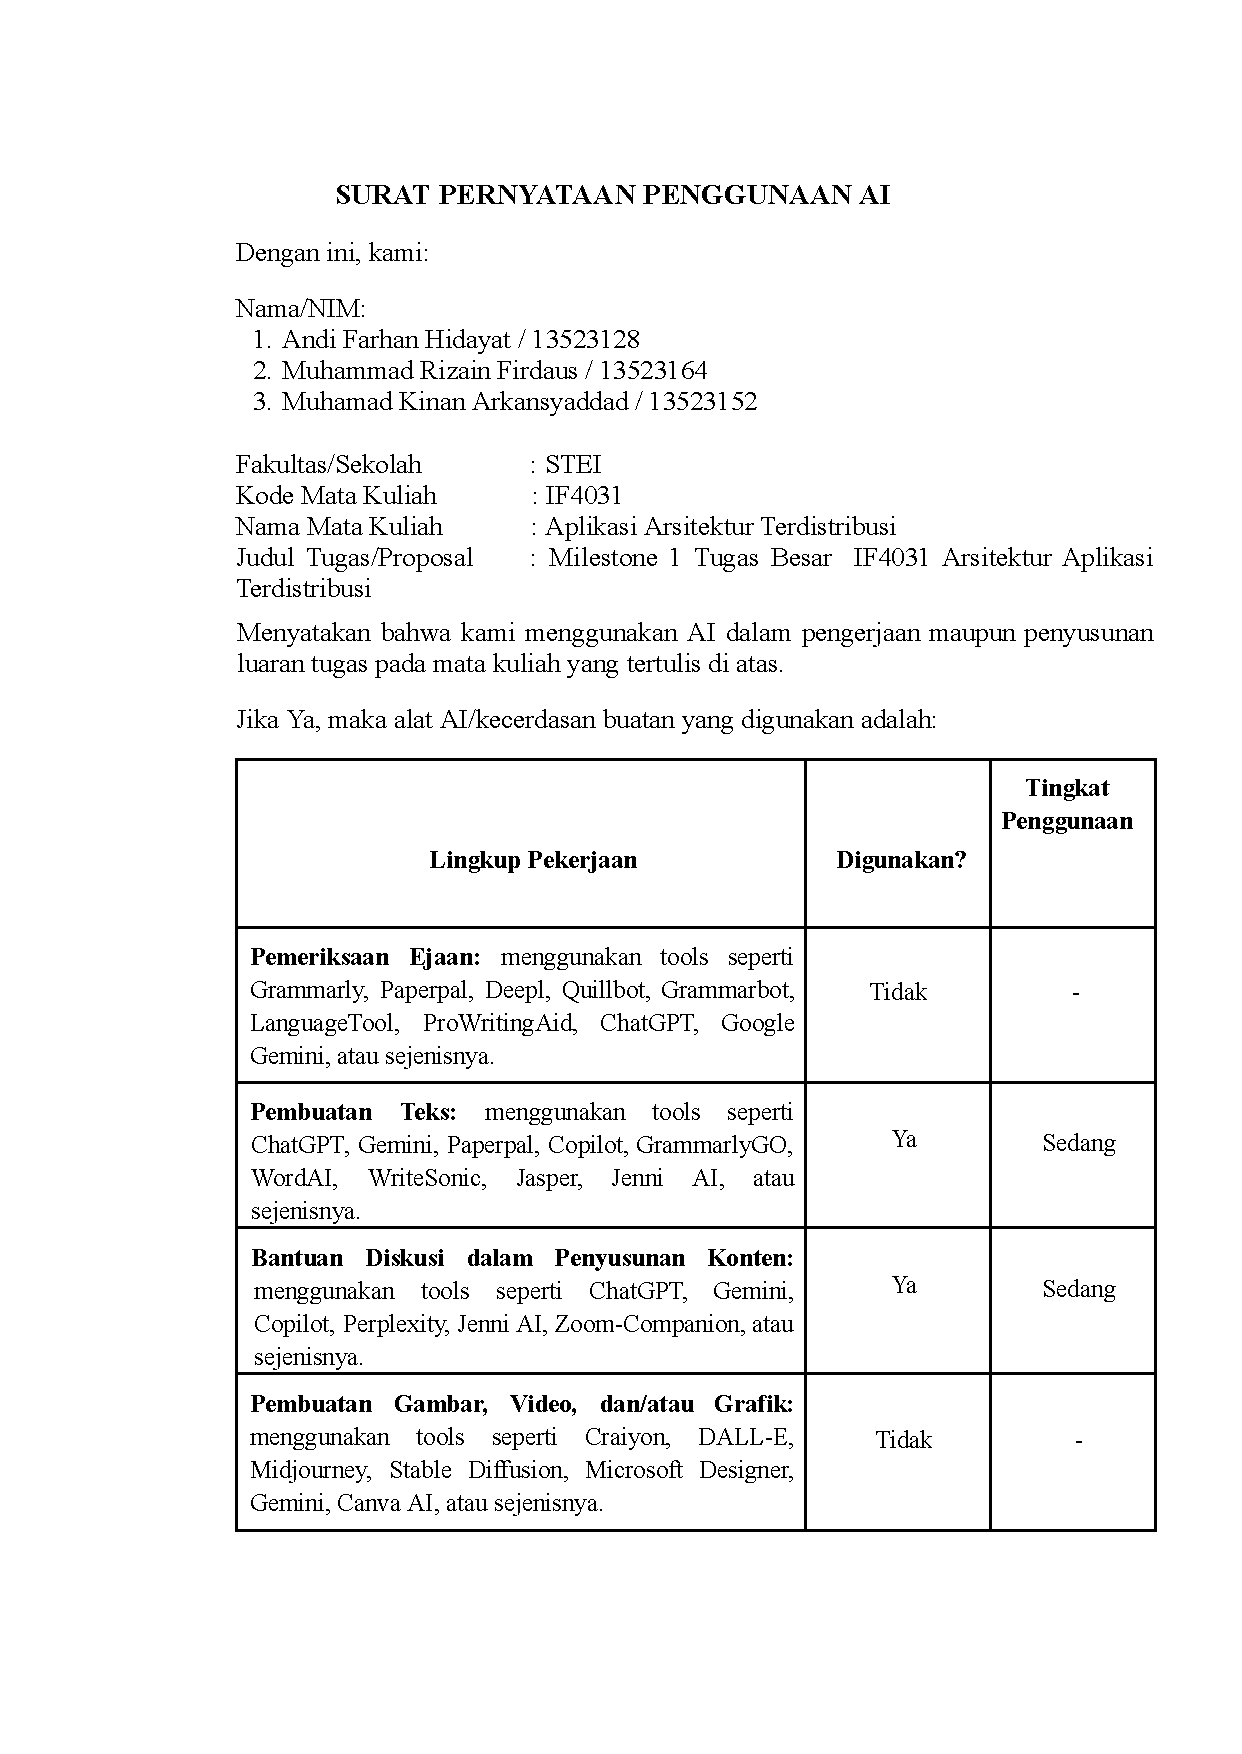
\includepdf[pages=-,pagecommand={\thispagestyle{empty}}]{IF4031_Surat-Pernyataan-AI_OrangSuksesAamiin.pdf}


\end{document}
